\documentclass[10pt, pdf, xcolor=pdftex, dvipsnames, table]{beamer}

\usepackage[brazil]{babel}
\usepackage[utf8]{inputenc}
\usepackage[T1]{fontenc}
\usepackage{amsfonts}
\usepackage{amsmath}
\usepackage{algorithm}
\usepackage{algpseudocode}
\usepackage{pgfpages}
\usepackage{fancyvrb}
\usepackage{times}
\usepackage{amsmath,amssymb}
\usepackage{graphicx}
\usepackage{hyperref}
\usepackage{pxfonts,txfonts}
\usepackage{url}
\usefonttheme{structurebold}
\usepackage{hyphenat}
\usepackage{multicol}
\usepackage{palatino}
\usepackage[normalem]{ulem}
\usepackage{booktabs}
\useunder{\uline}{\ul}{}
\usepackage{appendix}
\usepackage{float}
\usepackage{verbatim}
\usepackage{cooltooltips}
\usepackage{paralist}
\usepackage[inline]{enumitem}
\usepackage{multirow}
\usepackage{array}
\usepackage{xargs}
\usepackage{xcolor}
\usepackage{subfigure}
\usepackage{caption}
%\usepackage{bm}

\captionsetup{font=scriptsize,labelfont=scriptsize}
\captionsetup{skip=1pt,belowskip=1pt}

\definecolor{mygray}{gray}{0.8}

\newtheorem{hipotese}{Hipótese}

\usepackage{listings} % para inserir codigo fonte
\lstset{extendedchars=true,frame=tb,basicstyle=\footnotesize,stringstyle=\ttfamily,showstringspaces=true}

\renewcommand{\lstlistingname}{Listagem}

\newcommand{\x}{\textbf{\textcolor{Green}{$\surd$}}}
\newcommand{\xx}{\textbf{\textcolor{Blue}{$\odot$}}}
\newcommand{\xxx}{\textbf{\textcolor{Red}{$\times$}}}

\usetheme{Amsterdam}
\usefonttheme[onlymath]{serif}

\floatname{algorithm}{Algoritmo}

\newenvironment<>{varblock}[2][.9\textwidth]{%
\setlength{\textwidth}{#1}
	\begin{actionenv}#3%
    		\def\insertblocktitle{#2}%
    		\par%
    		\usebeamertemplate{block begin}}
  		{\par%
    		\usebeamertemplate{block end}%
  	\end{actionenv}}

% Efeitos:
\transdissolve %dissolve a lamina anterior;
% \transsplitverticalout % a proxima lamina se abre como uma cortina no sentido horizontal;
% \transblindshorizontal % a lamina anterior converte-se linha a linha.

% Para gerar apenas as páginas sem efeitos de overlay use (bom para imprimir):
% \usepackage[handout]{beamer}

% Para colocar número de páginas no slide:
%\setbeamertemplate{footline}[frame number]

% Para retirar a barra de navegação:
\setbeamertemplate{navigation symbols}{}

% inserir logotipo a apresentação
\pgfdeclareimage[height=1.5cm]{logo}{images/lups_oficial.png}
\logo{\pgfuseimage{logo}}

% Ativa ou desativa as anotações
\setbeameroption{hide notes}
%\setbeameroption{show notes}

%==================================================================================

%EVENTO
\renewcommand{\evento}{Apresentação de artigo - Metodologia para pesquisa e desenvolvimento em Computação }

% TITULO DA APRESENTACAO
\title{Cloud service selection using cloud service brokers: approaches and challenges}

%Autor
\author{Meysam Vakili $^{1}$
\and Neda Jahangiri $^{1}$
\and Mohsen Sharifi $^{2}$
\newline
\newline
\and Apresentador: Maicon Ança dos Santos
}

%%%%%%%%%%%%%%%%%%%%%%%%%%%%%%%%%%%%%%%%
% Instituição , 
%%%%%%%%%%%%%%%%%%%%%%%%%%%%%%%%%%%%%%%%

\institute{1\quad Department of Computer Engineering, University of Science and Culture, Tehran, Iran \\ 2\quad School of Computer Engineering, Iran University of Science and Technology, Tehran, Iran
}

\date{\today}

\begin{document}

\frame{\titlepage}
\pgfdeclareimage[height=0.7cm]{logo}{images/lups_timbre.png}
\logo{\pgfuseimage{logo}}
%\frame{\tableofcontents}


%%%%%%%%%%%%%%%%%%%%%%%%%%%%%%%%%%%%%%%%%%%%%
% Conteúdo da Apresentação
%%%%%%%%%%%%%%%%%%%%%%%%%%%%%%%%%%%%%%%%%%%%%

\section[Introdução]{Introdução}

%\begin{frame}
%	\tableofcontents[currentsection]
%\end{frame}

\begin{frame}
	\frametitle{Introdução}
	\begin{block}{}
		\begin{itemize}
		    \item[•] Usuários de computação em nuvem se deparam com uma ampla variedade de serviços para escolher;
		    \newline
		    \item[•] Surgimento de vários brokers de serviços em nuvem (CSBs) para ajudar os usuários em seu processo de seleção de serviços;
		    \newline
		    \item[•] A escolha do CSB por um cliente pode ser fundamental para a eficácia dos serviços de computação em nuvem.
		\end{itemize}
	\end{block}
\end{frame}

\begin{frame}
	\frametitle{Introdução}
	\begin{block}{}
		\begin{itemize}
		    \item[•] Um CSB é um serviço que atua em nome de um cliente no provisionamento de recursos e \textit{deploy};
		    \newline
		    \item[•] Gerencia \textbf{\textcolor{blue}{uso}}, \textbf{\textcolor{blue}{desempenho}} e \textbf{\textcolor{blue}{entrega}} dos serviços de nuvem;
		    \newline
		    \item[•] É o mediador da negociação entre provedores e consumidores.
		\end{itemize}
	\end{block}
\end{frame}

\begin{frame}
	\begin{figure}[htbp]
		\centerline{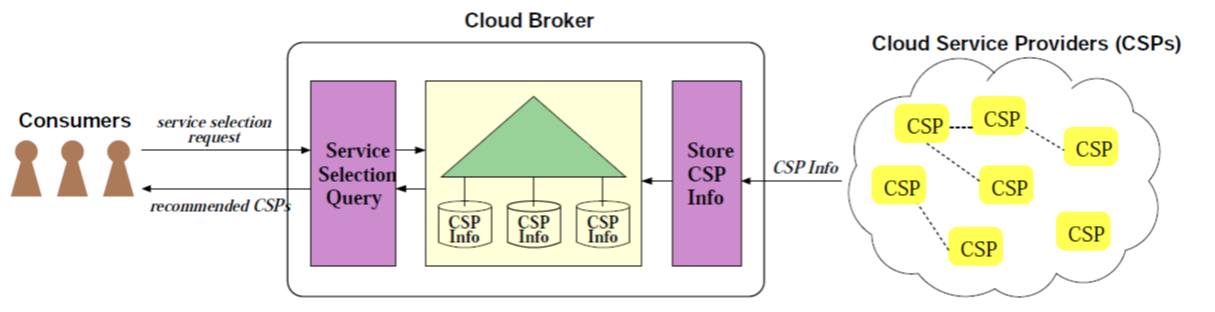
\includegraphics[scale=0.27]{images/CSBv2.png}}
		\caption[An Overview of the Cloud Broker Service]{An Overview of the Cloud Broker Service}
	\end{figure}
\end{frame}

%	
%	\subsection*{Aplicações Bag of Tasks}
%	
%	\begin{frame}
%		\begin{block}{\textit{Bag of Tasks}}
%			\begin{itemize}
%				\item[•] São aplicações paralelas cujas tarefas são independentes entre si \cite{Cirne2003};
%				\item[•] Mineração de dados, simulações, buscas massivas e muitas outras aplicações científicas com alta demanda de processamento;
%				\item[•] A arquitetura geral é composta de um servidor de tarefas e nós processadores.
%			\end{itemize}
%		\end{block}
%	\end{frame}
%	
%	\begin{frame}
%		\begin{figure}[htbp]
%			\centerline{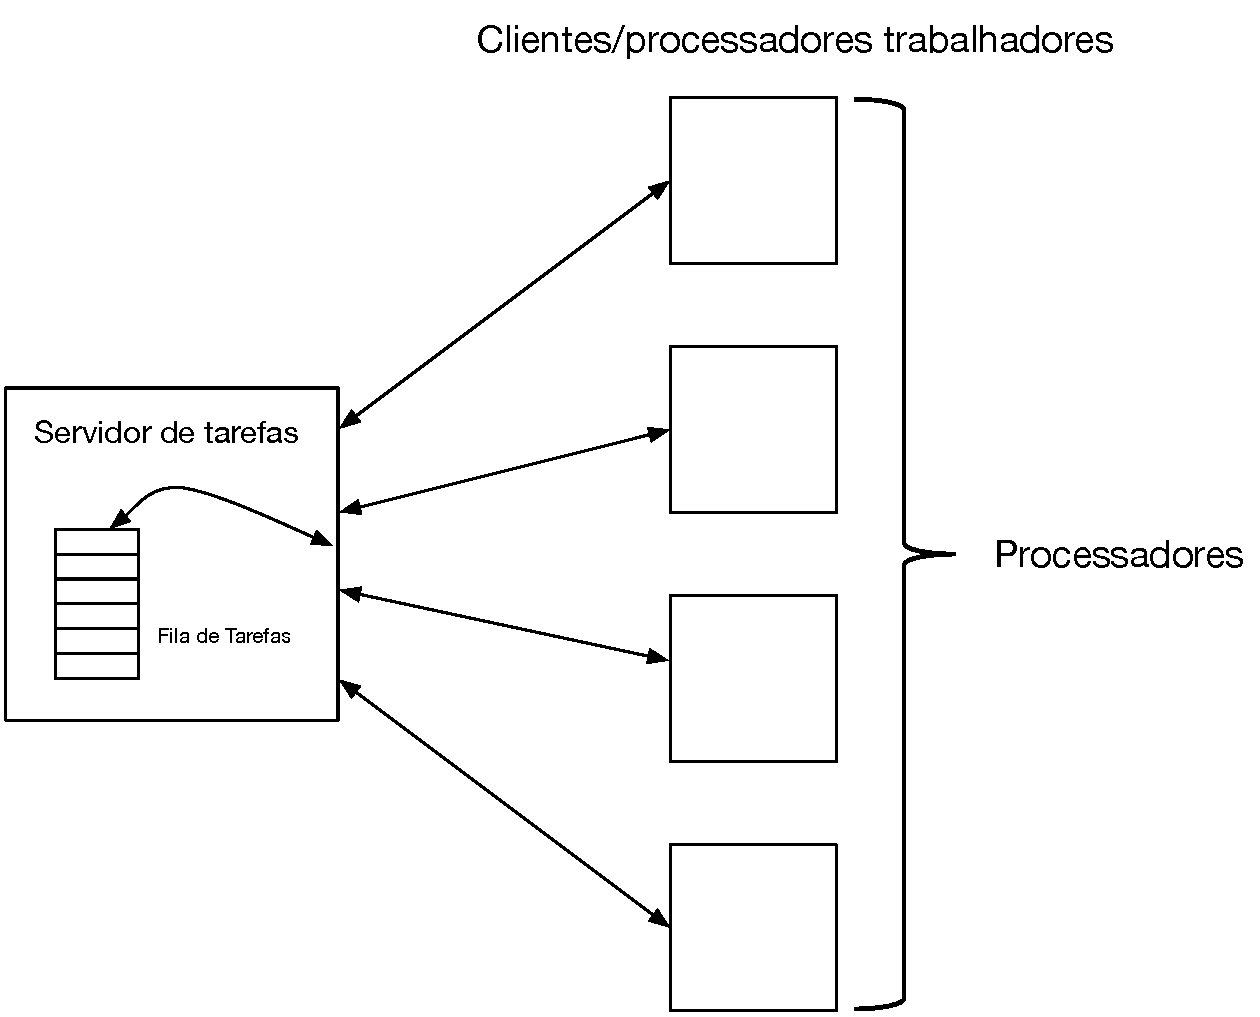
\includegraphics[scale=.4]{images/Bot.pdf}}
%			\caption{Modelo de controle centralizado para \textit{Bag of Tasks}.}
%			\label{BagOfTasks}
%		\end{figure}
%	\end{frame}
%	
%	\subsection*{Computação em Nuvem}
%	
%	\begin{frame}
%		\begin{block}{Computação em Nuvem}
%			\begin{itemize}
%				\item[•] Modelo que permite o acesso de rede a recursos compartilhados e configuráveis \cite{Mell};
%				\item[•] Servidores, armazenamento, aplicações, serviços;
%				\item[•] Modelos SaaS, PaaS e IaaS (este último, utilizado no trabalho).
%			\end{itemize}
%		\end{block}
%	\end{frame}
%		
%	\subsection*{OpenStack}
%	
%	\begin{frame}
%		\begin{block}{OpenStack}
%			\begin{itemize}
%				\item[•] Tecnologia de computação em nuvem que produz uma plataforma ubíqua \textit{open-source} para nuvens públicas e privadas \cite{Hu2013};
%				\item[•] Plataforma composta por vários módulos de software que geram uma nuvem IaaS;
%				\item[•] Módulos instalados: \textit{Keystone}, \textit{Glance}, \textit{Nova}, \textit{Nova-network} e \textit{Horizon}.
%			\end{itemize}
%		\end{block}
%	\end{frame}
%	
%	\begin{frame}
%		\begin{figure}[htbp]
%			\centerline{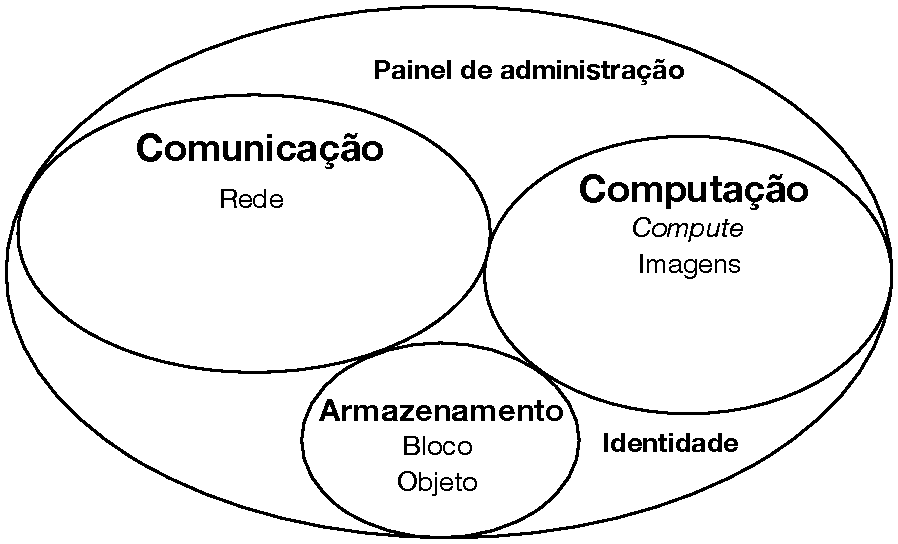
\includegraphics[scale=.50]{images/openstack_mainservices2.pdf}}
%			\caption[Principais serviços do OpenStack]{Principais serviços do OpenStack. Adaptado de \cite{Litvinski2013a}.}
%			\label{fig:openstackmainservices}
%		\end{figure}
%	\end{frame}
	
\section[Atributos de um CSB efetivo]{Atributos de um CSB efetivo}

\begin{frame}
	\tableofcontents[currentsection]
\end{frame}

\begin{frame}
	\frametitle{Atributos de um CSB efetivo}
	\begin{block}{}
		\begin{itemize}
		    \item[•] Suporte para vários atributos de QoS
		    	\begin{itemize}
		    		\item[-] \footnotesize\textit{disponibilidade, segurança, desempenho, escalabilidade, confiabilidade}
		    	\end{itemize}
		    \item
		    \item[•] Reconhecimento de violação de SLA
		    	\begin{itemize}
		    		\item[-] \footnotesize\textit{identificar violações, tomar as medidas adequadas e compensar prejuízos acumulados.}
		    	\end{itemize}
		    \item
		    \item[•] Otimização de preços:
		    	\begin{itemize}
		    		\item[-] \footnotesize\textit{vial na decisão, os CSBs devem considerar importante na seleção.}
		    	\end{itemize}
		\end{itemize}
	\end{block}
\end{frame}

\begin{frame}
	\frametitle{Atributos de um CSB efetivo}
	\begin{block}{}
		\begin{itemize}
		    \item[•] Seleção de fornecedores adequados para diferentes tipos de
serviços na nuvem
				\begin{itemize}
		    		\item[-] \footnotesize\textit{everything as a service (XaaS); o CSB deve conhecer e pesquisar em todos}
		    	\end{itemize}
		    \item
		    \item[•] Perfil do cliente
		    	\begin{itemize}
		    		\item[-] \footnotesize\textit{problema de pesquisa: perfil ou histórico de solicitações acelera o processo }
		    	\end{itemize}
		    \item
		    \item[•] Corretagem dinâmica
		    	\begin{itemize}
		    		\item[-] \footnotesize\textit{O CSB deve selecionar o melhor serviço em função da dinâmica}
		    	\end{itemize} 
		\end{itemize}
	\end{block}
\end{frame}

\begin{frame}
	\frametitle{Atributos de um CSB efetivo}
	\begin{block}{}
		\begin{itemize}
		    \item[•] Pedido parcial de informação sobre especificação de serviços
dos clientes
				\begin{itemize}
		    		\item[-] \footnotesize\textit{os CSBs devem mediar entre os provedores e clientes menos profissionais}
		    	\end{itemize}
		    \item
		    \item[•] Priorização de preferência do cliente
		    	\begin{itemize}
		    		\item[-] \footnotesize\textit{as prioridades dos clientes devem ser consideradas na seleção dos serviços}
		    	\end{itemize}
		\end{itemize}
	\end{block}
\end{frame}

\section[Cloud service brokers]{Cloud service brokers}

\begin{frame}
	\tableofcontents[currentsection]
\end{frame}

\begin{frame}
	\frametitle{Cloud Service Brokers}
	\begin{block}{}
		\begin{itemize}
		    \item[•] Single service model
				\begin{itemize}
		    		\item[-] \footnotesize\textit{suportam o modelo de serviço SaaS, mas pode suportar outros modelos}
		    	\end{itemize}
		    \item
		    \item[•] Multiple service model
		    	\begin{itemize}
		    		\item[-] \footnotesize\textit{suportam mais de um modelo de serviço em nuvem: flexibilidade}
		    	\end{itemize}
		\end{itemize}
	\end{block}
\end{frame}

\begin{frame}
	\frametitle{Cloud service brokers}
	\begin{table}[]
		\centering
		\caption{Classificação de CSBs revisados}
		\label{my-label}
		\resizebox{\textwidth}{!}{%
		\begin{tabular}{cc}
			\hline
			\textbf{Single service model} & \textbf{Multiple service model} \\ \hline
QBROKAGE & AHP \& TOPSIS \\
SLA-based SaaS Provisioning & CSP-index \\
Brokering Using Game Theory & Two Layered Brokerage \\
STRATOS & SMICloud \\
Distributed Cloud Brokering & Brokering for Optimized Placement of Virtual Machines \\
Multi-Cloud Brokering & OWL-S Based Semantic CSB \\
Dynamic Brokering on Federated Clouds & Price Optimization using 0-1 Knapsack \\
T-Broker &  \\ \hline
		\end{tabular}%
	}
	\end{table}
\end{frame}

\section[Principais desafios]{Principais desafios}

\begin{frame}
	\tableofcontents[currentsection]
\end{frame}

\begin{frame}
	\frametitle{Desafios comuns	}
	\begin{block}{}
		\begin{itemize}
		    \item[•] Não há suporte para vários modelos de serviço em nuvem:
				\begin{itemize}
		    		\item[-] \footnotesize\textit{o CSB deve ser capaz de encontrar provedores adequados para todos os tipos de serviço}
		    	\end{itemize}
		    \item
		    \item[•] Nenhum suporte desejável para atributos de QoS
		    	\begin{itemize}
		    		\item[-] \footnotesize\textit{o CSB deve suportar todos os atributos de QoS no momento da seleção do serviço}
		    	\end{itemize}
		\end{itemize}
	\end{block}
\end{frame}

\begin{frame}
	\begin{table}[]
		\centering
		\caption{CSB approaches (single service model)}
		\label{my-label}
		\resizebox{\textwidth}{!}{%
		\begin{tabular}{cll}
			\hline
		\textbf{Approaches} & \multicolumn{1}{c}{\textbf{Main contributions}} & \multicolumn{1}{c}{\textbf{Main challenges}} \\ \hline
QBROKAGE & \begin{tabular}[c]{@{}l@{}}1. Modeling applications, resources \\ and QoS attributes in OVF format;\\ 2. Making an application graph based \\ on OVF file;\\ 3. Using game theory to map \\ applications to providers.\end{tabular} & \begin{tabular}[c]{@{}l@{}}1. Only uses commercial provider \\ information;\\ 2. Is not elastic to support previously \\ deployed applications.\end{tabular} \\
\multicolumn{1}{l}{} &  &  \\
Multi-cloud brokering & \begin{tabular}[c]{@{}l@{}}1. Using a scheduler to deploy \\ VMs in clouds;\\ 2. Using a VM manager for monitoring \\ and updating the VM list;\\ 3. Using a cloud manager for updating \\ the instance list and dynamic\\ pricing\end{tabular} & \begin{tabular}[c]{@{}l@{}}1. Only price, efficiency, and energy \\ consumption are considered in service selection\\ 2. Receiving much professional \\ information from users in the service\\ description file\end{tabular} \\ \hline
\end{tabular}%
}
\end{table}
\end{frame}

\begin{frame}
	\begin{table}[]
		\centering
		\caption{CSB approaches (multiple service model)}
		\label{my-label}
		\resizebox{\textwidth}{!}{%
		\begin{tabular}{cll}
			\hline
			\textbf{Approaches}                                                                  & \multicolumn{1}{c}{\textbf{Main contributions}}                                                                                                                                                                                                                                            & \multicolumn{1}{c}{\textbf{Main challenges}}                                                                                                                                                                                            \\ \hline
Two layers brokering                                                                 & \begin{tabular}[c]{@{}l@{}}1. Using two brokers: \\ SaaS broker and cloud broker\\ 2. To create communication between \\ brokers in two phases: discovery and binding\\ 3. To define the efficiency property based \\ on cloud broker information to assess \\ SaaS providers\end{tabular} & \begin{tabular}[c]{@{}l@{}}1. Only availability, reliability and \\ response time are considered \\ in service selection\\ 2. High rate of network communications \\ when the number of SaaS and \\ IaaS providers is high\end{tabular} \\
\multicolumn{1}{l}{}                                                                 &                                                                                                                                                                                                                                                                                            &                                                                                                                                                                                                                                         \\
		\begin{tabular}[c]{@{}c@{}}Brokering for\\ optimized placement\\ of VMs\end{tabular} & \begin{tabular}[c]{@{}l@{}}1. Using cloud scheduler to supply an \\ optimized deployment plan for VMs\\ 2. Using a virtual infrastructure manager \\ to deploy each VM on a selected cloud\end{tabular}                                                                                    & \begin{tabular}[c]{@{}l@{}}1. It is not quantifiable in case of dynamic \\ service allocation\\ 2. Differences in the performances of \\ virtual machine managers\\ is not considered			\end{tabular}                                      \\ \hline
		\end{tabular}%
	}
	\end{table}
\end{frame}

%\begin{frame}
%	\frametitle{Cloud Service Brokers}
%	\begin{block}{}
%		\begin{itemize}
%		    \item[•] Single service model
%				\begin{itemize}
%		    		\item[-] \footnotesize\textit{suporta o modelo de serviço SaaS, mas pode suportar outros modelos}
%		    	\end{itemize}
%		    \item
%		    \item[•] Multiple service model
%		    	\begin{itemize}
%		    		\item[-] \footnotesize\textit{suportam mais de um modelo de serviço em nuvem: flexibilidade}
%		    	\end{itemize}
%		\end{itemize}
%	\end{block}
%\end{frame}

\section[Avaliação e comparação]{Avaliação e comparação}

\begin{frame}
	\tableofcontents[currentsection]
\end{frame}

\begin{frame}
\begin{table}[]
\centering
\caption{Comparison of represented approaches based on the proposed attributes of an effective CSB}
\label{my-label}
\resizebox{\textwidth}{!}{%
\begin{tabular}{lcccccccc}
\hline
\multicolumn{1}{c}{\textbf{Approaches}}                                            & \textbf{\begin{tabular}[c]{@{}c@{}}Qos attributes\\ used\end{tabular}}                 & \textbf{\begin{tabular}[c]{@{}c@{}}SLA violation\\ determination\end{tabular}} & \textbf{\begin{tabular}[c]{@{}c@{}}Price\\ optimizing\\ mechanism\end{tabular}} & \textbf{\begin{tabular}[c]{@{}c@{}}Cloud\\ service\\ model\\ selection\end{tabular}} & \textbf{\begin{tabular}[c]{@{}c@{}}Using user\\ profile\end{tabular}}                               & \textbf{\begin{tabular}[c]{@{}c@{}}Dynamic/\\ Static\\ brokering\end{tabular}} & \textbf{\begin{tabular}[c]{@{}c@{}}Quantity \&\\ quality of\\ information\\ received from\\ user\end{tabular}} & \textbf{\begin{tabular}[c]{@{}c@{}}Prioritize\\ customer\\ preferences\end{tabular}} \\ \hline
QBROKAGE                                                                           & \begin{tabular}[c]{@{}c@{}}Commercial\\ providers QoS\end{tabular}                     & No                                                                             & No                                                                              & IaaS                                                                                 & No                                                                                                  & D                                                                              & Balanced                                                                                                       & No                                                                                   \\
                                                                                   & \multicolumn{1}{l}{}                                                                   & \multicolumn{1}{l}{}                                                           & \multicolumn{1}{l}{}                                                            & \multicolumn{1}{l}{}                                                                 & \multicolumn{1}{l}{}                                                                                & \multicolumn{1}{l}{}                                                           & \multicolumn{1}{l}{}                                                                                           & \multicolumn{1}{l}{}                                                                 \\
\begin{tabular}[c]{@{}l@{}}Multi-cloud\\ brokering\end{tabular}                    & \begin{tabular}[c]{@{}c@{}}Cost,\\ Performance \&\\ Energy consumption\end{tabular}    & No                                                                             & Yes                                                                             & IaaS                                                                                 & \begin{tabular}[c]{@{}c@{}}Yes - by\\ historical\\ profile of the\\ deployed\\ service\end{tabular} & D                                                                              & \begin{tabular}[c]{@{}c@{}}Too Muchand\\ Professional\end{tabular}                                             & No                                                                                   \\
                                                                                   & \multicolumn{1}{l}{}                                                                   & \multicolumn{1}{l}{}                                                           & \multicolumn{1}{l}{}                                                            & \multicolumn{1}{l}{}                                                                 & \multicolumn{1}{l}{}                                                                                & \multicolumn{1}{l}{}                                                           & \multicolumn{1}{l}{}                                                                                           & \multicolumn{1}{l}{}                                                                 \\
Two layers brokering                                                               & \begin{tabular}[c]{@{}c@{}}Availability,\\ Reliability \&\\ Response time\end{tabular} & No                                                                             & No                                                                              & Multiple                                                                             & No                                                                                                  & D                                                                              & Balanced                                                                                                       & No                                                                                   \\
                                                                                   & \multicolumn{1}{l}{}                                                                   & \multicolumn{1}{l}{}                                                           & \multicolumn{1}{l}{}                                                            & \multicolumn{1}{l}{}                                                                 & \multicolumn{1}{l}{}                                                                                & \multicolumn{1}{l}{}                                                           & \multicolumn{1}{l}{}                                                                                           & \multicolumn{1}{l}{}                                                                 \\
\begin{tabular}[c]{@{}l@{}}Brokering for optimized\\ placement of VMs\end{tabular} & \begin{tabular}[c]{@{}c@{}}Performance, Cost\\ \& Load balance\end{tabular}            & No                                                                             & Yes                                                                             & Multiple                                                                             & No                                                                                                  & S                                                                              & Balanced                                                                                                       & No                                                                                   \\ \hline
\end{tabular}%
}
\end{table}
\end{frame}

%
%	\subsection*{Modelo de Aplicação BoT}
%	
%	\begin{frame}
%		\begin{block}{Descrição de aplicação BoT}
%			\begin{equation*}
%				\resizebox{.9\hsize}{!}{$A = \{q_1 \dots q_n\} ~\textsf{onde}~ q_i = [a_i,d_i,b_i,c_i], \forall  i ~ | ~ 1 \le  i \le n$}
%			\end{equation*}
%			\newline
%			{\footnotesize
%			\begin{itemize}
%				\item $a$: instante de tempo no qual o conjunto de tarefas chega para o processamento;
%				\item $d$: tempo de duração do grupo de tarefas. A unidade de tempo é o \textit{passo};
%				\item $b$: quantidade de tarefas descritas por quádrupla;
%				\item $c$: taxa de utilização de CPU para cada tarefa da quádrupla.
%			\end{itemize}}
%		\end{block}
%	\end{frame}
%	
%	\begin{frame}
%		\begin{block}{Exemplo de aplicação BoT}
%			\begin{equation*}
%				\resizebox{.9\hsize}{!}{$A = \{[0,5,3,50],[0,8,5,30],[3,4,6,80],[4,10,2,20]\}$}
%			\end{equation*}
%			\newline
%			{\footnotesize
%			Uma aplicação $A$ composta de um total de 16 tarefas, distribuídas em quatro grupos idênticos. Os dois primeiros grupos definem tarefas que chegam no tempo 0 (zero) do processamento. As tarefas do terceiro e do quarto grupo são adicionadas ao \emph{bag} nos tempos 3 e 4.}
%		\end{block}
%	\end{frame}
%	
%	\begin{frame}
%		\begin{equation*}
%			\resizebox{.9\hsize}{!}{$A = \{\textbf{[0, 5, 3, 50], [0, 8, 5, 30]},\textcolor{mygray}{[3, 4, 6, 80], [4, 10, 2, 20]}\}$}
%		\end{equation*}
%		\begin{figure}[htbp]
%			\centerline{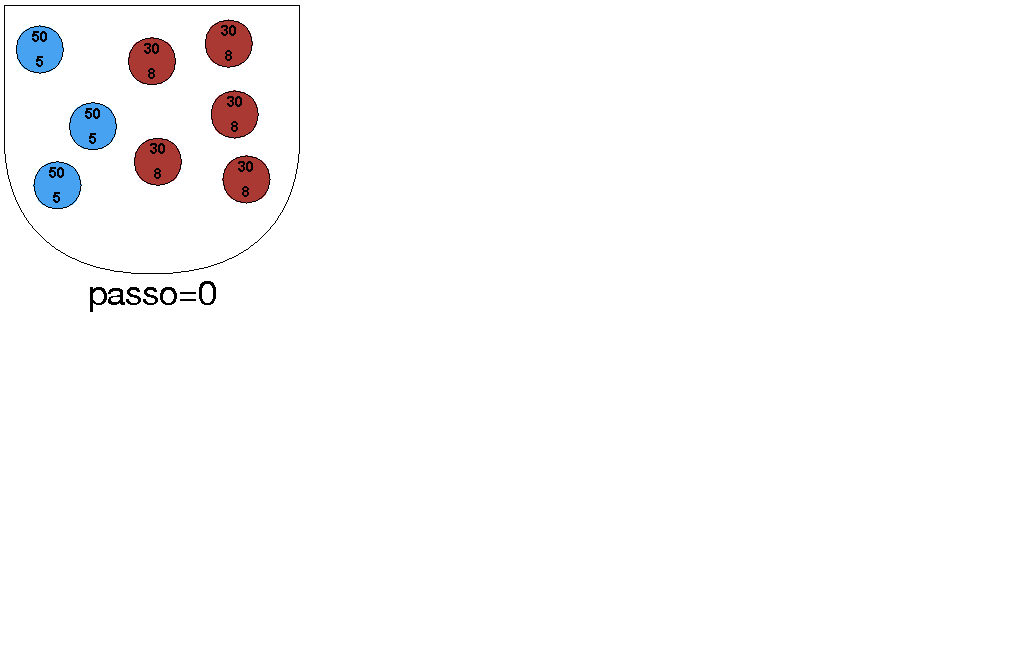
\includegraphics[scale=0.55]{images/BagOfTasks4-1.pdf}}
%			\caption[Exemplo de aplicação \textit{Bag of Tasks}]{Exemplo de aplicação \textit{Bag of Tasks}.}
%			\label{fig:exemplobot4-1}
%		\end{figure}
%	\end{frame}
%	
%	\begin{frame}
%		\begin{equation*}
%			\resizebox{.9\hsize}{!}{$A = \{\textbf{[0, 5, 3, 50], [0, 8, 5, 30]},\textcolor{mygray}{[3, 4, 6, 80], [4, 10, 2, 20]}\}$}
%		\end{equation*}
%		\begin{figure}[htbp]
%			\centerline{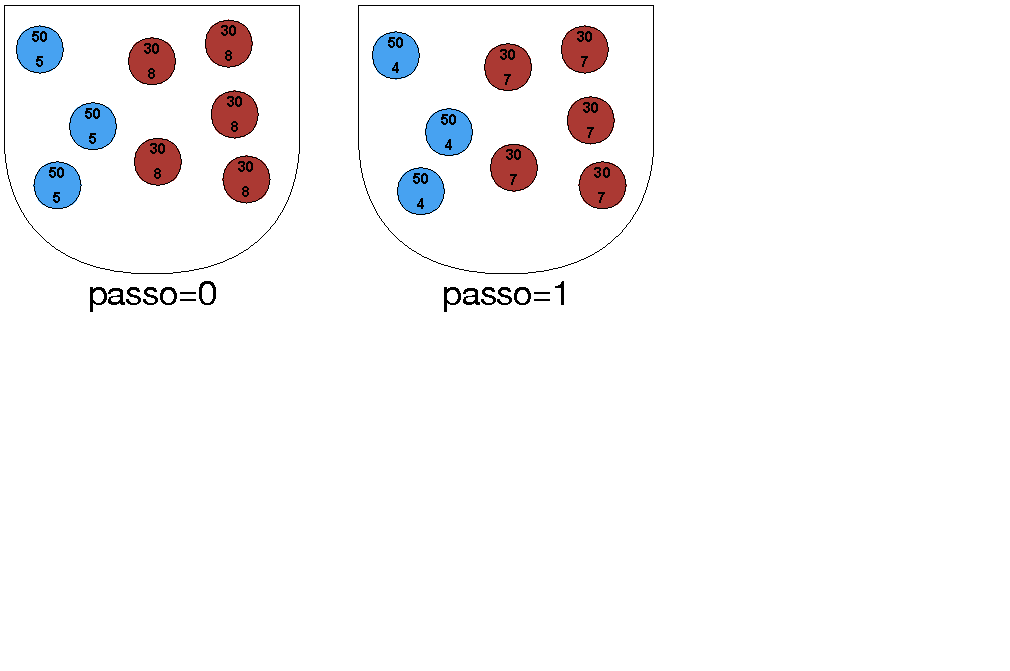
\includegraphics[scale=0.55]{images/BagOfTasks4-2.pdf}}
%			\caption[Exemplo de aplicação \textit{Bag of Tasks}]{Exemplo de aplicação \textit{Bag of Tasks}.}
%			\label{fig:exemplobot4-2}
%		\end{figure}
%	\end{frame}
%	
%	\begin{frame}
%		\begin{equation*}
%			\resizebox{.9\hsize}{!}{$A = \{\textbf{[0, 5, 3, 50], [0, 8, 5, 30]},\textcolor{mygray}{[3, 4, 6, 80], [4, 10, 2, 20]}\}$}
%		\end{equation*}
%		\begin{figure}[htbp]
%			\centerline{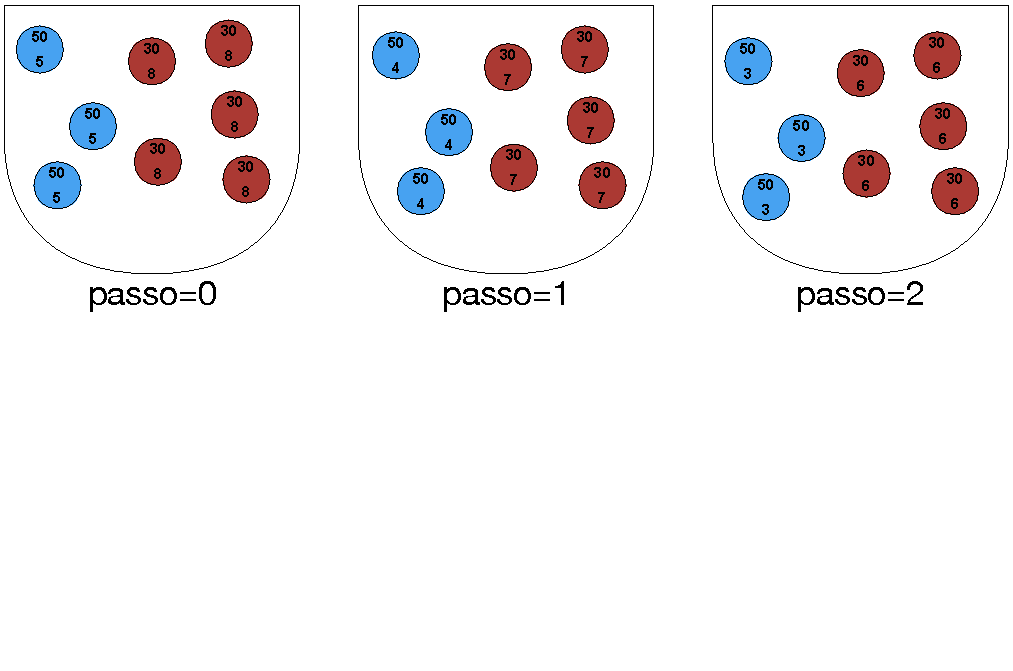
\includegraphics[scale=0.55]{images/BagOfTasks4-3.pdf}}
%			\caption[Exemplo de aplicação \textit{Bag of Tasks}]{Exemplo de aplicação \textit{Bag of Tasks}.}
%			\label{fig:exemplobot4-3}
%		\end{figure}
%	\end{frame}
%	
%	\begin{frame}
%		\begin{equation*}
%			\resizebox{.9\hsize}{!}{$A = \{\textbf{[0, 5, 3, 50], [0, 8, 5, 30], [3, 4, 6, 80]}, \textcolor{mygray}{[4, 10, 2, 20]}\}$}
%		\end{equation*}
%		\begin{figure}[htbp]
%			\centerline{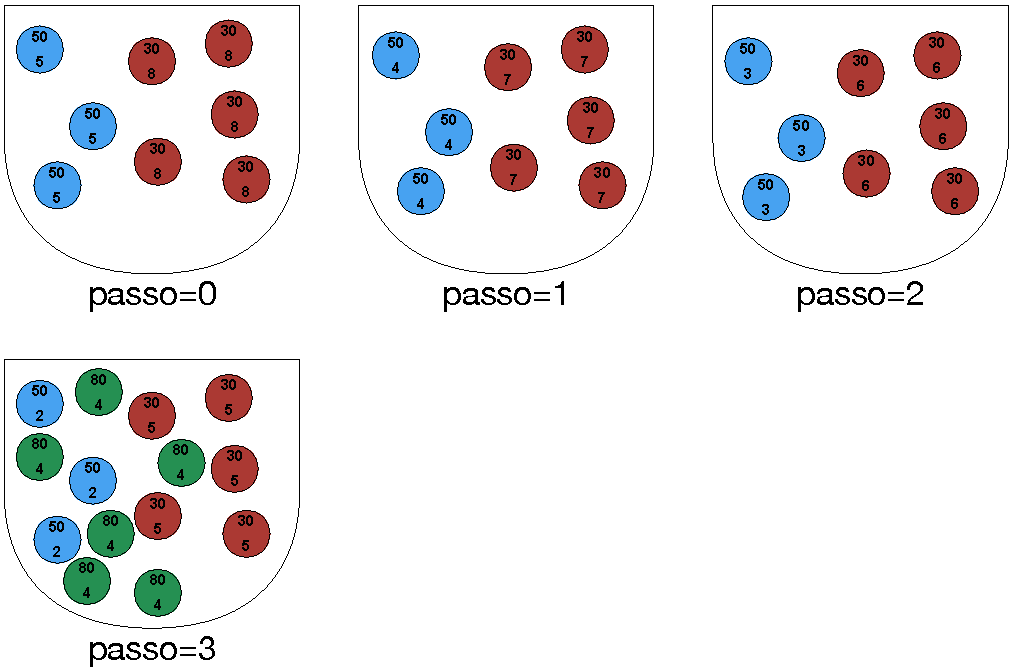
\includegraphics[scale=0.55]{images/BagOfTasks4-4.pdf}}
%			\caption[Exemplo de aplicação \textit{Bag of Tasks}]{Exemplo de aplicação \textit{Bag of Tasks}.}
%			\label{fig:exemplobot4-4}
%		\end{figure}
%	\end{frame}
%	
%	\begin{frame}
%		\begin{equation*}
%			\resizebox{.9\hsize}{!}{$A = \{\textbf{[0, 5, 3, 50], [0, 8, 5, 30], [3, 4, 6, 80], [4, 10, 2, 20]}\}$}
%		\end{equation*}
%		\begin{figure}[htbp]
%			\centerline{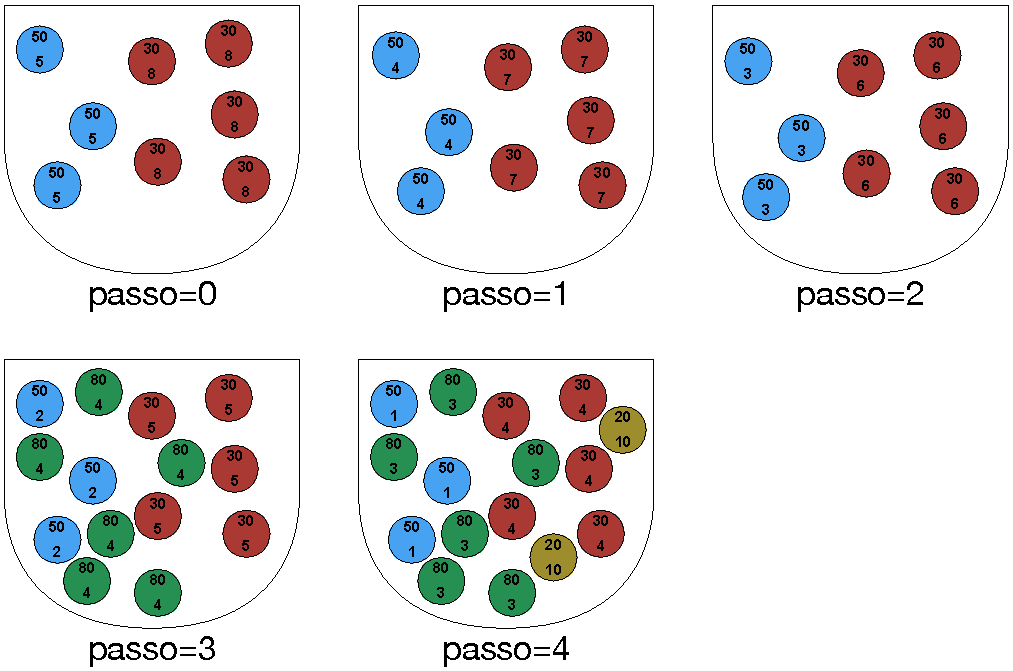
\includegraphics[scale=0.55]{images/BagOfTasks4-5.pdf}}
%			\caption[Exemplo de aplicação \textit{Bag of Tasks}]{Exemplo de aplicação \textit{Bag of Tasks}.}
%			\label{fig:exemplobot4-5}
%		\end{figure}
%	\end{frame}
%	
%	\begin{frame}
%		\begin{equation*}
%			\resizebox{.9\hsize}{!}{$A = \{\textcolor{mygray}{[0, 5, 3, 50]}, \textbf{[0, 8, 5, 30], [3, 4, 6, 80], [4, 10, 2, 20]}\}$}
%		\end{equation*}
%		\begin{figure}[htbp]
%			\centerline{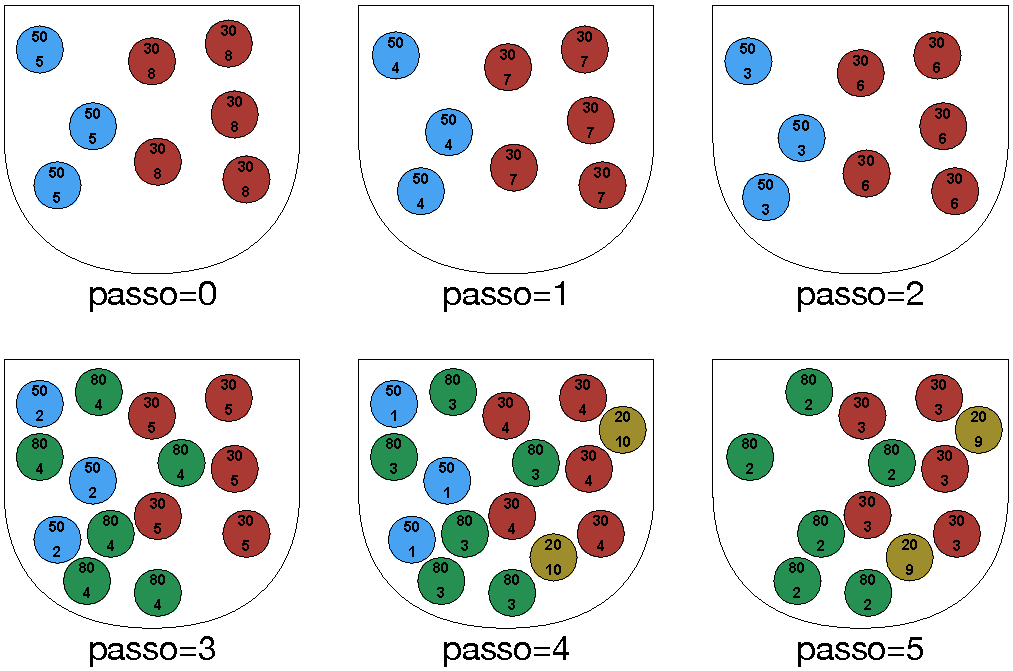
\includegraphics[scale=0.55]{images/BagOfTasks4-6.pdf}}
%			\caption[Exemplo de aplicação \textit{Bag of Tasks}]{Exemplo de aplicação \textit{Bag of Tasks}.}
%			\label{fig:exemplobot4-6}
%		\end{figure}
%	\end{frame}
%		
%	\subsection*{Consolidação de Tarefas}
%	
%	\begin{frame}
%		\begin{block}{}
%			\begin{itemize}
%				\item[•] Define-se \emph{passo} a passagem de uma unidade de tempo;
%				\begin{itemize}
%					\item[-] a duração $d_i$ de uma tarefa $\tau_i$ descreve o número de passos necessários para executá-la;
%				\end{itemize}
%				\item[•] Ao conjunto de instruções de passo de uma tarefa se dá o nome de \emph{job};
%				\begin{itemize}
%					\item[-] cada \textit{job} possui um \textit{timestep} de 300 segundos (valor definido para este trabalho).
%				\end{itemize}
%				\item[•] Uma tarefa é composta por um sequência de \textit{jobs}.
%			\end{itemize}
%		\end{block}
%	\end{frame}
%	
%	\begin{frame} %\x antes deste slide, falar que a tarefa é composta por uma sequência de jobs, um job por timestep
%		\begin{block}{Conjunto de \textit{jobs} de uma tarefa}
%			\begin{equation*}
%				\resizebox{1\hsize}{!}{$\{w_1^i, w_2^i, \dots w_{d_i}^i\} = \{[g_1^i,r_1^i,f_1^i,c_1^i],[g_2^i,r_2^i,f_2^i,c_2^i], [g_3^i,r_3^i,f_3^i,c_3^i], \dots [g_{d_i}^i,r_{d_i}^i,f_{d_i}^i,c_{d_i}^i]\}$}
%			\end{equation*}
%			\newline
%			{\footnotesize
%			Sequência de \textit{jobs} da tarefa $i$, com $d_i$ \textit{timesteps}. Note que:
%			\begin{itemize}
%				\item $c^i_j$ do \textit{job} é igual a $c_i$ da tarefa;
%				\item $f^i_j + r^i_j = d_i$;
%				\item $g^i_j = a^i + f^i_j$ (mas quando tem contenção, $g^i_j \ge a^i + f^i_j$)
%			\end{itemize}}
%		\end{block}
%	\end{frame}
%	
%	\subsection*{Escalonamento Aplicativo}
%		
%	\begin{frame}
%		\begin{center}
%			\scalebox{0.7}
%			{
%				\begin{minipage}{1\linewidth}
%					\begin{algorithm}[H]
%						\caption{Consolidação de uma lista de tarefas em um conjunto de processadores.}
%						\label{algo:schedconsolida}
%						\begin{algorithmic}[1]
%							\Procedure{ConsolidaTarefas$<F>$}{$L,m',P,g$}
%								\State $L' \leftarrow \forall w_i \in L | g_i = g$
%								\State $L \leftarrow L - L'$
%								\State $L' \leftarrow Sort<F>(L')$
%								\If {$P = Lote$} %\Comment {Alocação por lote}
%									%\For {$i \leftarrow 1$ \textbf{to} $m'$}
%										\State //executa alocação por lote
%									\Else %\Comment {Alocação cíclica}
%												\State //executa alocação cíclica
%								\EndIf
%								\State $L \leftarrow L \cup L'$
%						        \State $\forall w_i \in L, g_i \leftarrow g_i+1$
%								\State $M' \leftarrow \{|P_1|, \dots, |P_m'|\}$
%								\State \textbf{return} $L, M'$
%							\EndProcedure
%						\end{algorithmic}
%					\end{algorithm}
%				\end{minipage}
%			}
%		\end{center}
%	\end{frame}
%	
%	\begin{frame}
%		\begin{center}
%			\scalebox{0.8}
%			{
%				\begin{minipage}{1\linewidth}
%					\begin{algorithm}[H]
%						\caption{Definição da prioridade de \textit{jobs} em função do custo computacional.}
%						\label{algo:funccrit1}			
%						\begin{algorithmic}[1]
%							\Procedure{$ComparaMaiorCusto$}{$w_i,w_j$}
%						      \If {$c_i \ge c_j$}
%						      \State \textbf{return} $true$
%						      \Else
%						      \State \textbf{return} $false$
%						      \EndIf
%						  	\EndProcedure
%						\end{algorithmic}
%					\end{algorithm}
%				\end{minipage}
%			}
%		\end{center}
%		\begin{block}{}
%			{\small
%				Dados dois \textit{jobs} $w_i$ e $w_j$, a função-critério $ComparaMaiorCusto$ retorna $true$ caso o custo de $w_i$ for maior que $w_j$ e $false$ caso contrário.
%			}
%		\end{block}
%	\end{frame}
%	
%	\begin{frame}
%		\begin{center}
%			\scalebox{0.8}
%			{
%				\begin{minipage}{1\linewidth}
%					\begin{algorithm}[H]
%						\caption{Definição da prioridade de \textit{jobs} em função da data de criação da tarefa.}
%						\label{algo:funccrit2}						
%						\begin{algorithmic}[1]
%							\Procedure{$ComparaTarefaMaisAntiga$}{$w_i,w_j$}
%						    	\If {$g_i-f_i  \ge g_j-f_j$}
%						      		\State \textbf{return} $true$
%						      \Else
%						      		\State \textbf{return} $false$
%						      \EndIf
%						  	\EndProcedure
%						\end{algorithmic}
%					\end{algorithm}
%				\end{minipage}
%			}
%		\end{center}
%		\begin{block}{}
%			{\small
%				Dados dois \textit{jobs} $w_i$ e $w_j$, a função-critério $ComparaTarefaMaisAntiga$ retorna $true$ caso a tarefa que tenha originado $w_i$ tenha completado um número maior de passos que $w_j$ e $false$, caso contrário.
%			}
%		\end{block}
%	\end{frame}
%	
%	\begin{frame}
%		\begin{block}{Exemplo de escalonamento aplicativo}
%			\begin{equation*}
%				\resizebox{.9\hsize}{!}{$A = \{[0, 2, 3, 20], [1, 4, 3, 30], [1, 2, 5, 50], [2, 2, 2, 60], [2, 3, 4, 40], [3, 1, 2, 80]\}$}
%			\end{equation*}
%			\newline
%			{\footnotesize
%			BoT descrevendo 19 tarefas distribuídas em 6 quádruplas. O total gerado é de 46 \textit{jobs}.}
%		\end{block}
%	\end{frame}
%	
%	\begin{frame}
%		\begin{figure}[htbp]
%			\centerline{
%			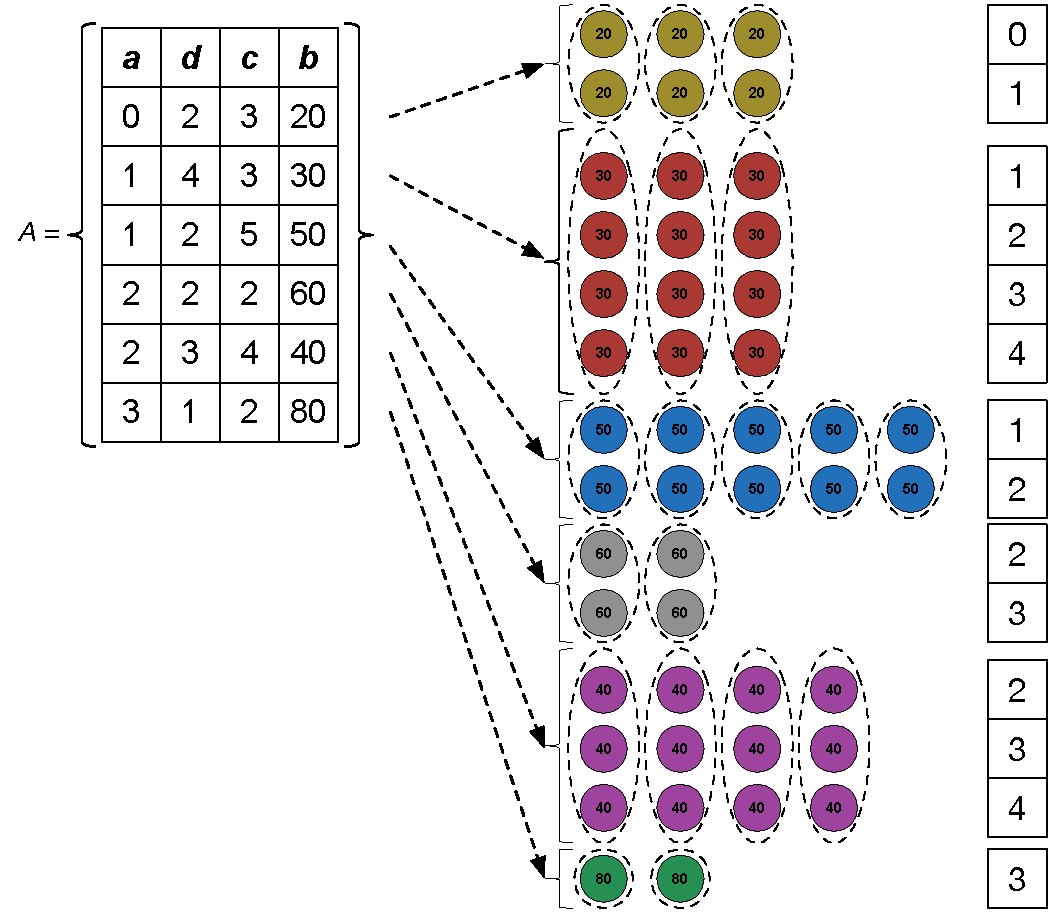
\includegraphics[scale=0.49]{images/EscalonamentoAplicativoNovo.pdf}}
%			\caption[Geração de \textit{jobs} a partir da descrição de uma aplicação BoT]{Geração de \textit{jobs} a partir da descrição de uma aplicação BoT.}
%			\label{fig:exemploescalonamentoaplicativonovo}
%		\end{figure}
%	\end{frame}
%	
%	\begin{frame}
%		\begin{figure}[htbp]
%			\centering
%			\subfigure[Ordenação por passo global]{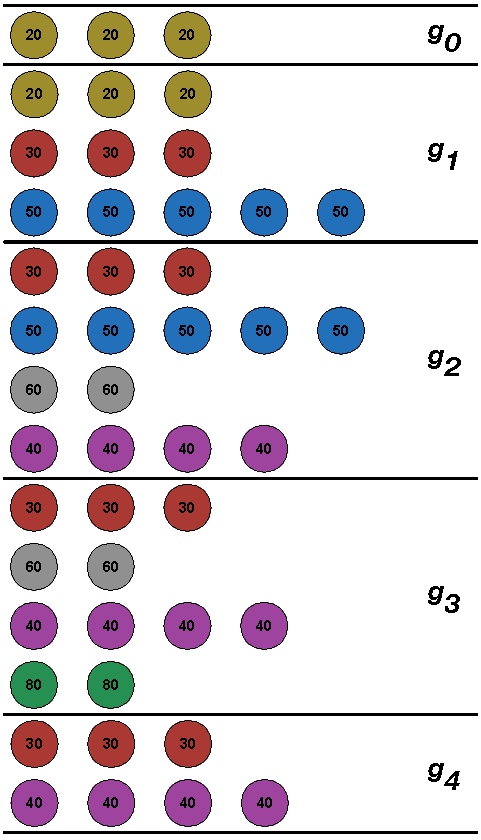
\includegraphics[scale=0.42]{images/EscalonamentoAplicativo1.pdf}}
%			\subfigure[Ordenação por função-critério (menor custo)]{	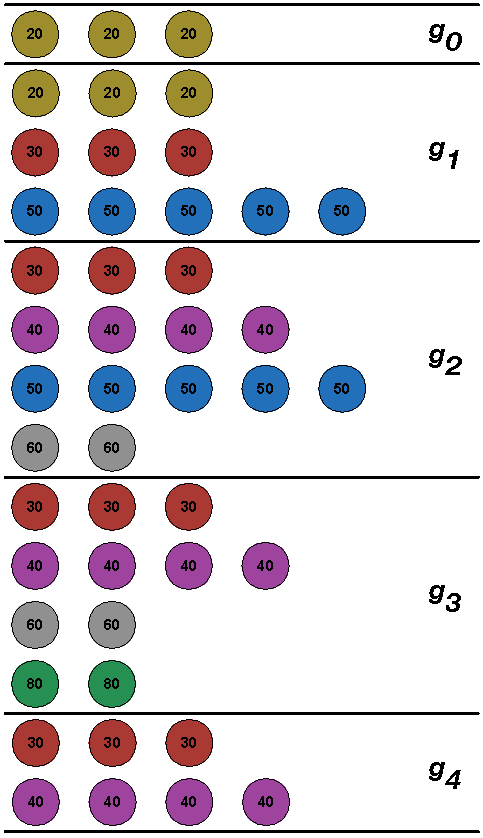
\includegraphics[scale=0.42]{images/EscalonamentoAplicativo2.pdf}}
%			\caption[Ordenação dos \textit{jobs} em função do passo global não contingenciado]{Ordenação dos \textit{jobs} em função do passo global não contingenciado.}
%			\label{fig:exemploescalonamentoaplicativo-2}
%		\end{figure}
%	\end{frame}
%	
%	\begin{frame}
%		\begin{figure}[htbp]
%			\centering
%			\subfigure[Alocação cíclica]{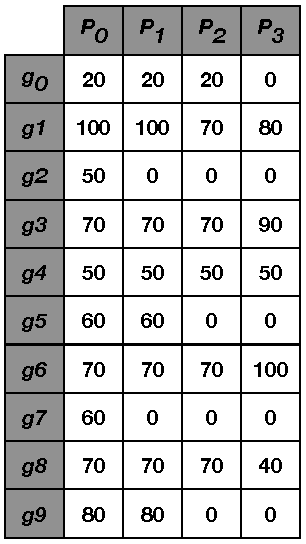
\includegraphics[scale=0.5]{images/EscalonamentoAplicativo3-2.pdf}}
%			\subfigure[Alocação por lote]{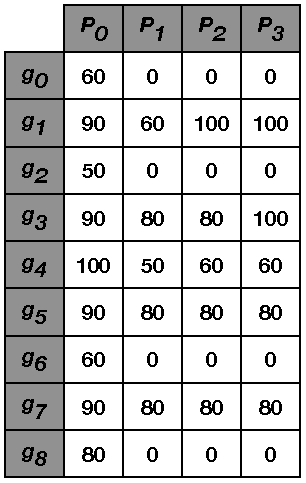
\includegraphics[scale=0.5]{images/EscalonamentoAplicativo4-2.pdf}}
%			\caption[Resultado final do escalonamento aplicativo]{Resultado final do escalonamento aplicativo.}
%			\label{fig:exemploescalonamentoaplicativo-3}
%		\end{figure}
%	\end{frame}
%	
%	\subsection*{Escalonamento Sistema}
%	
%	\begin{frame}
%		\begin{center}		
%			\scalebox{0.65}
%			{
%				\begin{minipage}{1\linewidth}
%					\begin{algorithm}[H]
%						\caption{Consolidação de máquinas virtuais.}
%						\label{algo:schedsisconsolida}
%						\begin{algorithmic}[1]
%							\Procedure{ConsolidaMVs$<G,H,I,J>$}{$M^{on},M^{off},\delta_h,\delta'_h,\delta_l,\delta'_l$}
%								\State $|M^{on}| = \sum_{i=0}^{m}|n_i|, iff~n_i \in M^{on} $
%						        \While {$\frac{|M^{on}|}{M^{on}.size} > \delta_h \land \exists n_i \in M^{off}$}
%						        \State $n^{aux} = M^{off}.first$
%						        \State $M^{off}.remove(n^{aux})$
%						        \State $M^{on}.insert(n^{aux})$
%						        \EndWhile
%						        \For {$n_i \leftarrow M^{on}.begin$ \textbf{to} $M^{on}.end$ \textbf{when} $|n_i| < \delta'_l$}
%						        \State $v \leftarrow \delta''_l - |n_i|$
%						        \State $n^{out} \leftarrow G(M^{on},v)$
%						        \State $|n_{out}| \leftarrow |n_{i}| + v$
%						        \State $|n_i| \leftarrow |n_i| - v$
%						        \EndFor
%								\textcolor{red}{\For {$n_{i} \leftarrow M^{on}.begin$ \textbf{to} $M^{on}.end$ \textbf{when} $|n_{aux}| > \delta'_h$}
%						        \State $v \leftarrow H(n_{i})$
%						        \State $n_{aux} \leftarrow I(M^{on}, v)$
%						        \State $|n_{i}| \leftarrow |n_{i}| - v$
%						        \State $|n_{aux}| \leftarrow |n_{aux}| + v$
%						        \EndFor}
%						        \For {$n_i \leftarrow M^{on}.begin$ \textbf{to} $M^{on}.end$ \textbf{when} $|n_i| < \delta_l$}
%						        \State $n^{in} \leftarrow J(M^{on},|n_i|)$
%						        \State $|n^{in}| \leftarrow |n^{in}| + |n_i|$
%						        \State $M^{on}.remove(n_i)$
%						        \State $M^{off}.insert(n_i)$
%						        \EndFor
%							\EndProcedure
%						\end{algorithmic}
%					\end{algorithm}			
%				\end{minipage}
%			}
%		\end{center}	
%	\end{frame}
%
%\section[Experimentação e Resultados]{Experimentação e Resultados}
%
%\begin{frame}
%	\tableofcontents[currentsection]
%\end{frame}
%
%	\subsection*{Ambiente de Testes}
%	
%	\begin{frame}
%		\begin{block}{Ambiente de Testes}
%			\begin{itemize}
%				\item[•] Um cluster formado por dez nós físicos;
%				\item[•] Cada nó equipado com:
%				\begin{itemize}
%					\item[•] 01 processador Intel Core i5-2310 @ 2.90GHz \textit{quad-core};
%					\item[•] 16GB de memória RAM;
%					\item[•] 01 interface de rede 1GbE;
%				\end{itemize}
%				\item[•] OpenStack com os módulos: \textit{Keystone}, \textit{Glance}, \textit{Compute}, \textit{Nova-network} e \textit{Horizon};
%				\item[•] OpenStack com escalonador padrão no qual somente uma estratégia é permitida e o mesmo atua no momento em que ocorre o lançamento das máquinas virtuais.
%			\end{itemize}
%		\end{block}
%	\end{frame}
%	
%	\subsection*{Metodologia dos Experimentos}
%
%	\begin{frame}
%		\begin{block}{Metodologia dos Experimentos}
%			\begin{itemize}
%				\item[•] Geração de BoT;
%				\item[•] Definição do número de processadores;
%				\item[•] Submissão de aplicações;
%				\item[•] Lançamento de máquinas virtuais;
%				\item[•] Coleta de dados.
%			\end{itemize}
%		\end{block}
%		\begin{block}{}
%			Um passo de execução equivale a 300 segundos (5 minutos), que é o tempo necessário para que sejam executadas 65000 \textit{bogo} operações, consumindo 100\% de CPU.
%		\end{block}
%	\end{frame}
%
%	\begin{frame}
%		\begin{block}{Metodologia dos experimentos}
%			\begin{table}[htbp]
%				\centering
%				\caption{Classificação proposta para BoTs neste trabalho.}
%				\label{tab:classenumquadruplas}
%				{\footnotesize
%				\begin{tabular}{lll}
%					\hline
%					\textbf{Classe} & \textbf{Características} & \textbf{Distribuição}     \\ \hline
%					$Q$           & Tamanho em termos de número de quádruplas & Fixa \\
%					$N$        & Número de tarefas por quádrupla & Weibull \\
%					$S$        & Duração para as tarefas & Normal\\ 
%					$L$        & Carga das tarefas& Normal \\
%					$I$        & Intervalo entre quádruplas& Weibull\\ \hline
%				\end{tabular}}
%			\end{table}
%		\end{block}
%	\end{frame}
%	
%	\begin{frame}
%		\begin{figure}[htbp]
%			\centerline{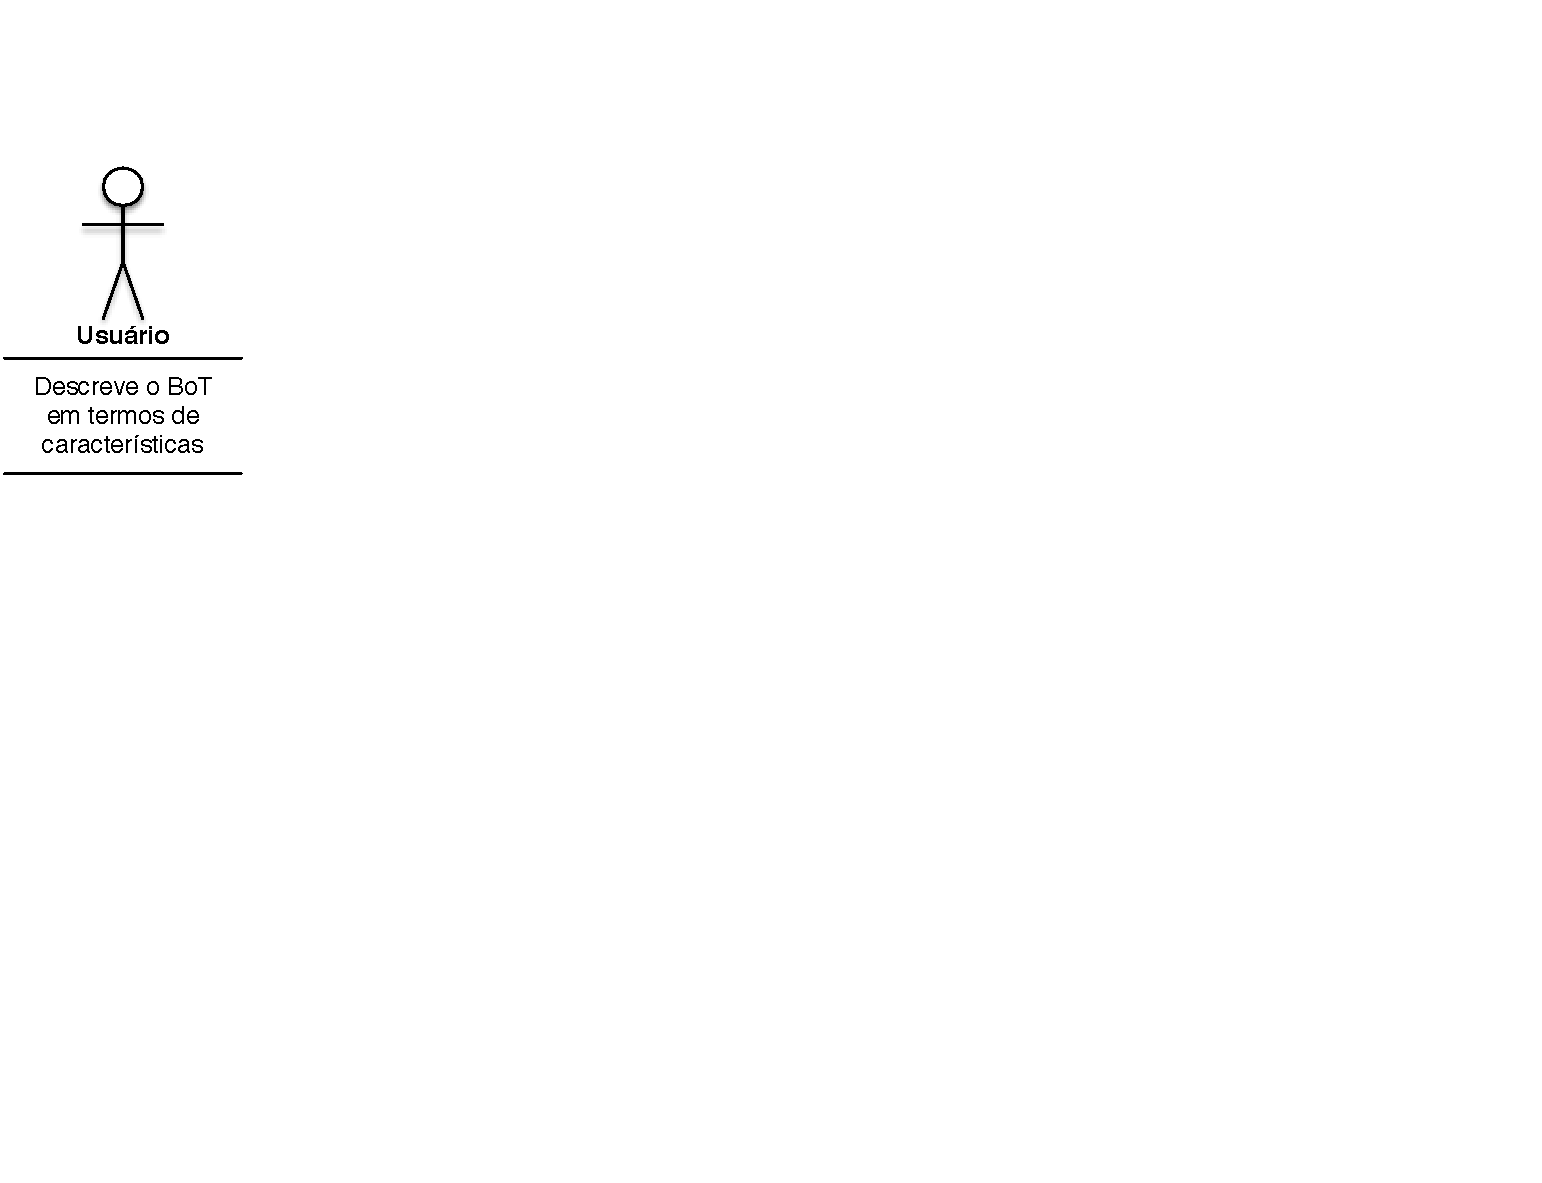
\includegraphics[scale=0.371]{images/ConsolidaTarefas1.pdf}}
%			\caption{Exemplo de descrição de BoT e comsolidação de tarefas.}
%			\label{fig:consolidatarefas1}
%		\end{figure}
%	\end{frame}
%	
%		\begin{frame}
%		\begin{figure}[htbp]
%			\centerline{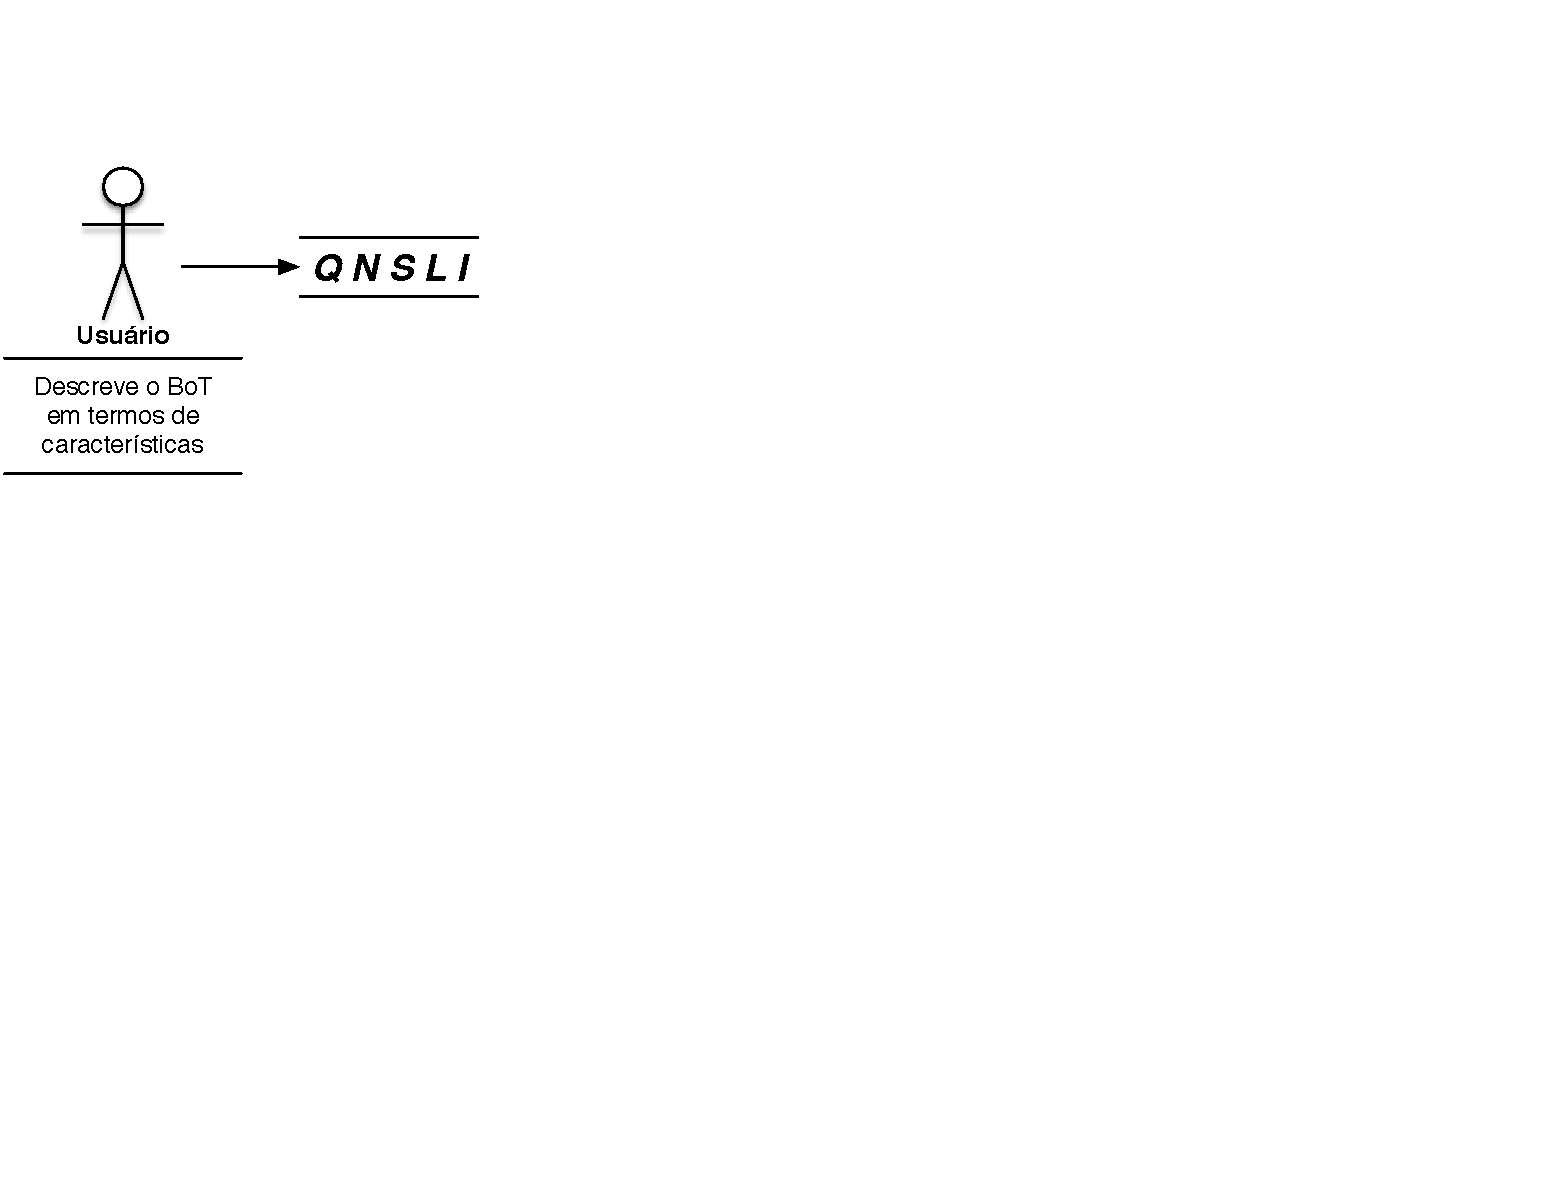
\includegraphics[scale=0.371]{images/ConsolidaTarefas2.pdf}}
%			\caption{Exemplo de descrição de BoT e comsolidação de tarefas.}
%			\label{fig:consolidatarefas2}
%		\end{figure}
%	\end{frame}
%
%	\begin{frame}
%		\begin{figure}[htbp]
%			\centerline{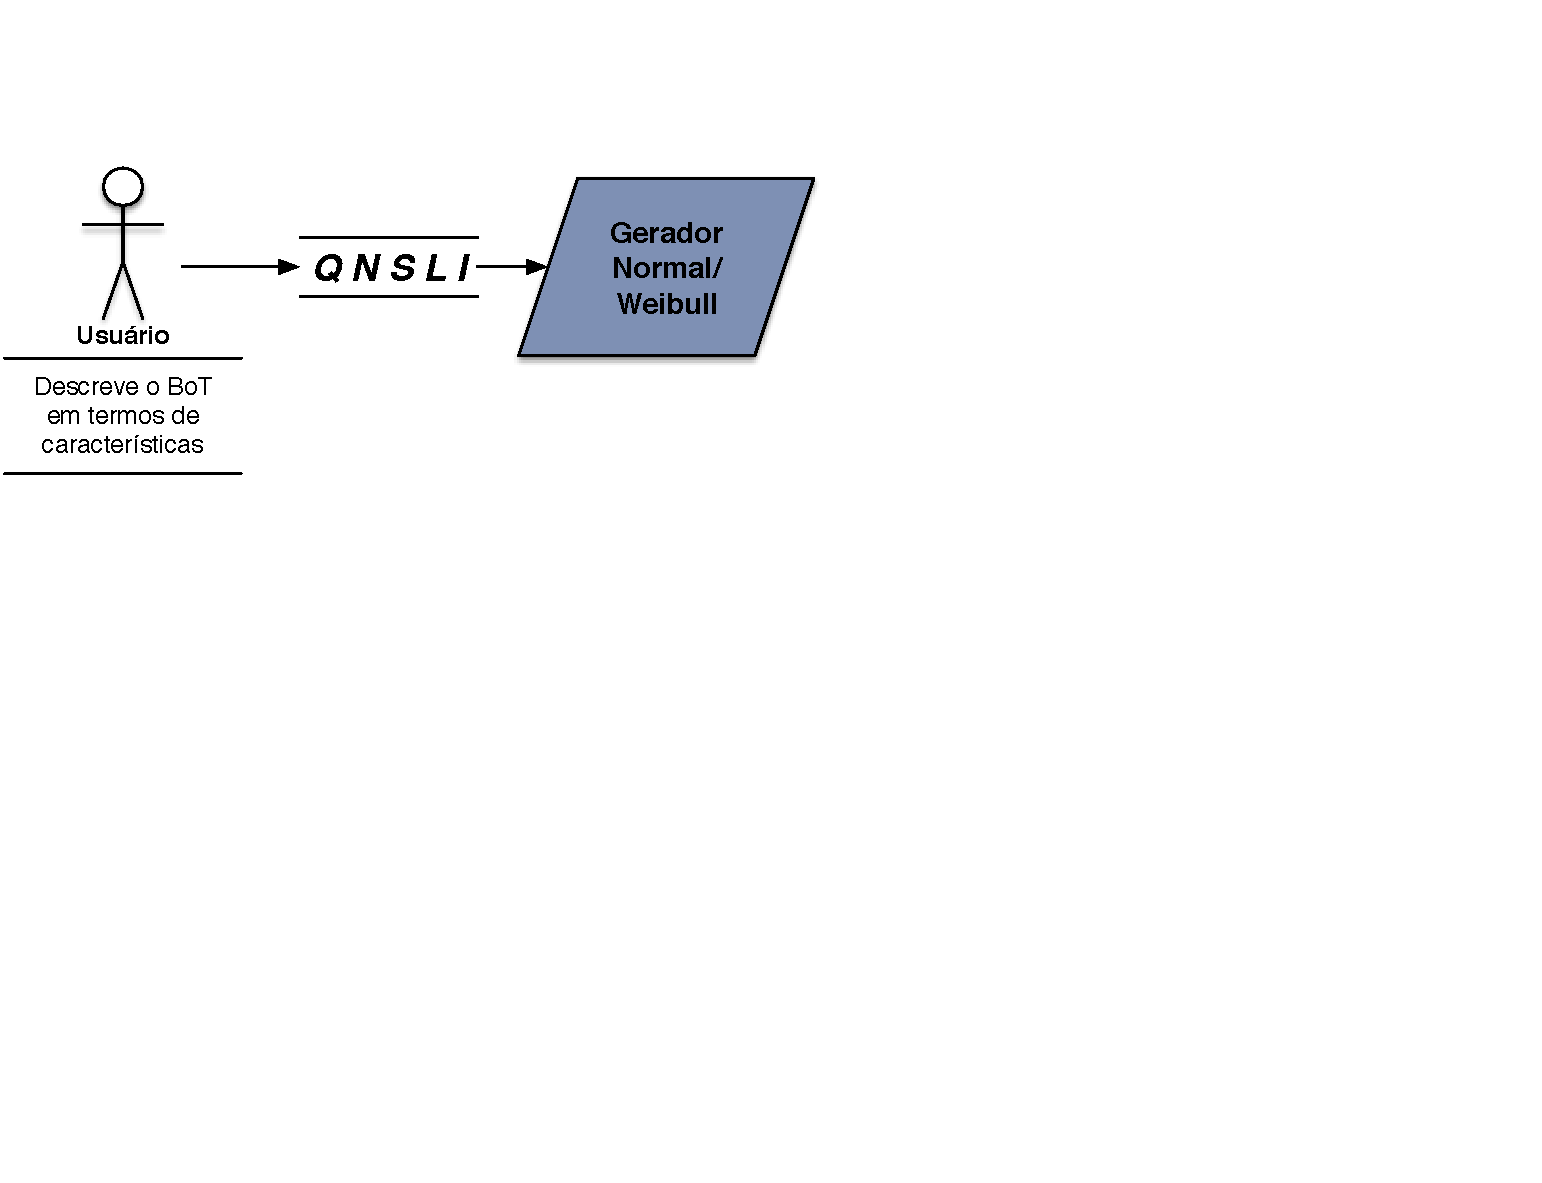
\includegraphics[scale=0.371]{images/ConsolidaTarefas3.pdf}}
%			\caption{Exemplo de descrição de BoT e comsolidação de tarefas.}
%			\label{fig:consolidatarefas3}
%		\end{figure}
%	\end{frame}
%
%	\begin{frame}
%		\begin{figure}[htbp]
%			\centerline{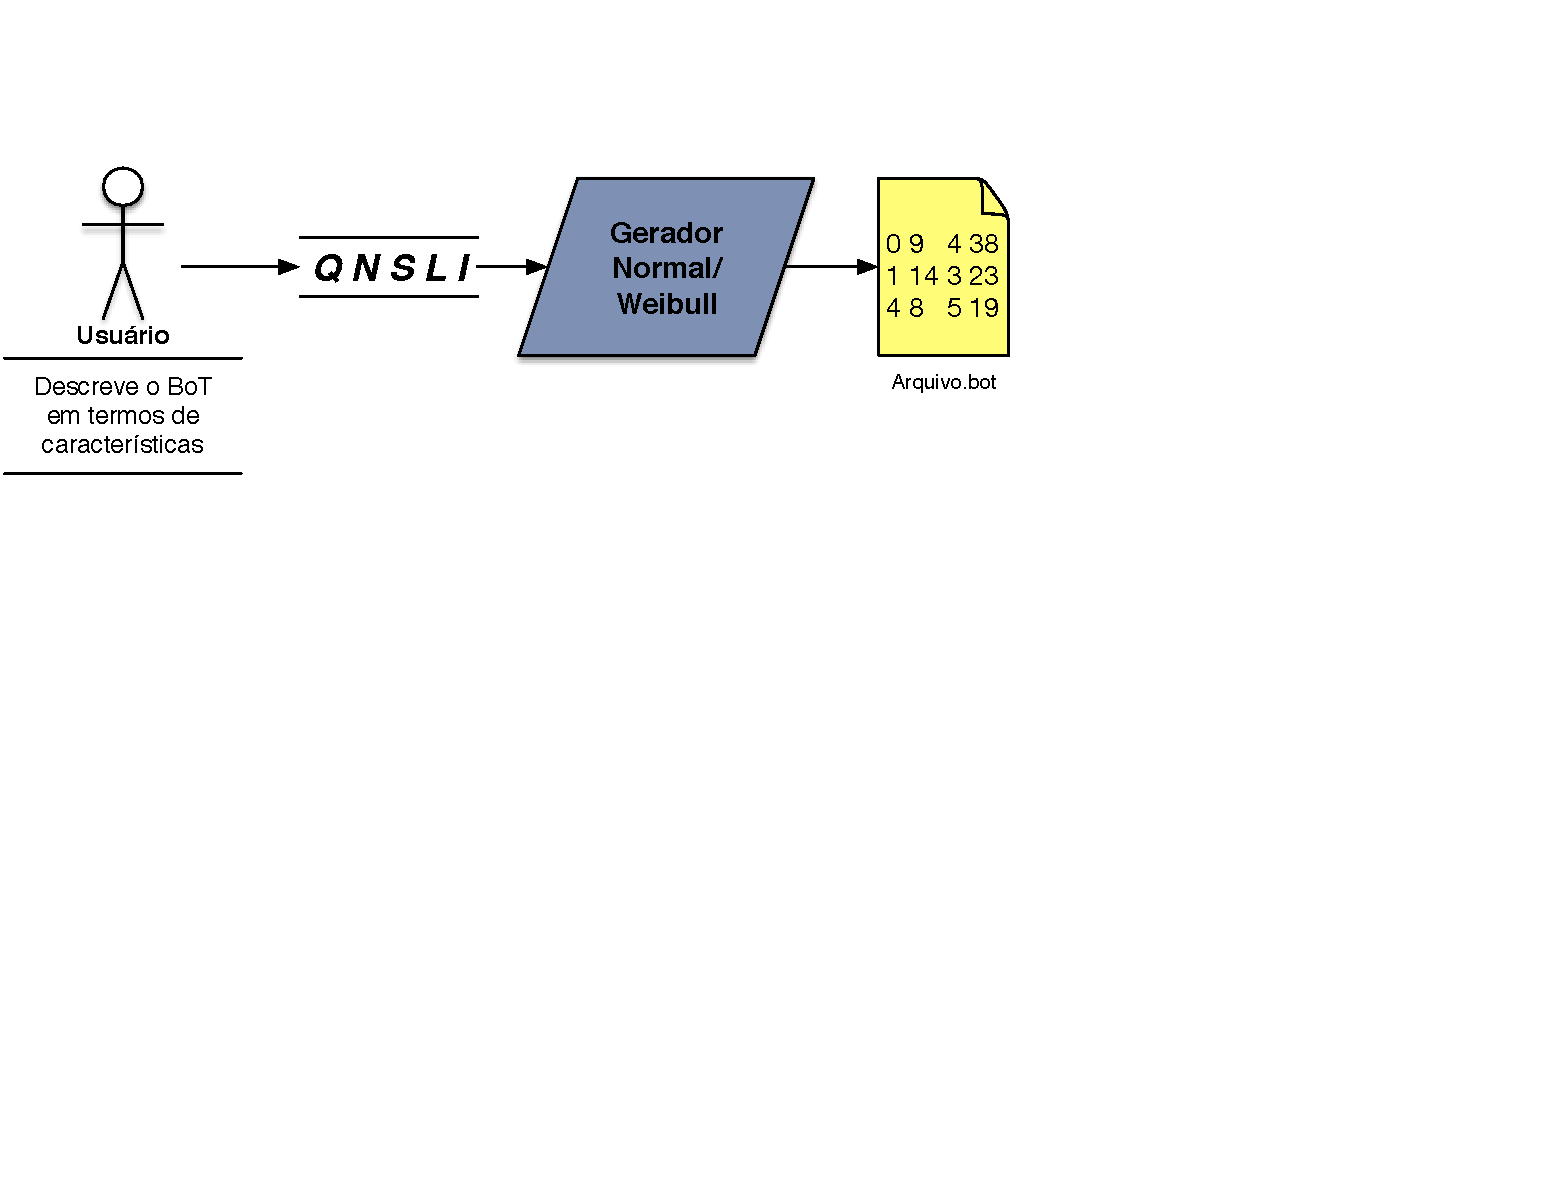
\includegraphics[scale=0.371]{images/ConsolidaTarefas4.pdf}}
%			\caption{Exemplo de descrição de BoT e comsolidação de tarefas.}
%			\label{fig:consolidatarefas4}
%		\end{figure}
%	\end{frame}
%
%	\begin{frame}
%		\begin{figure}[htbp]
%			\centerline{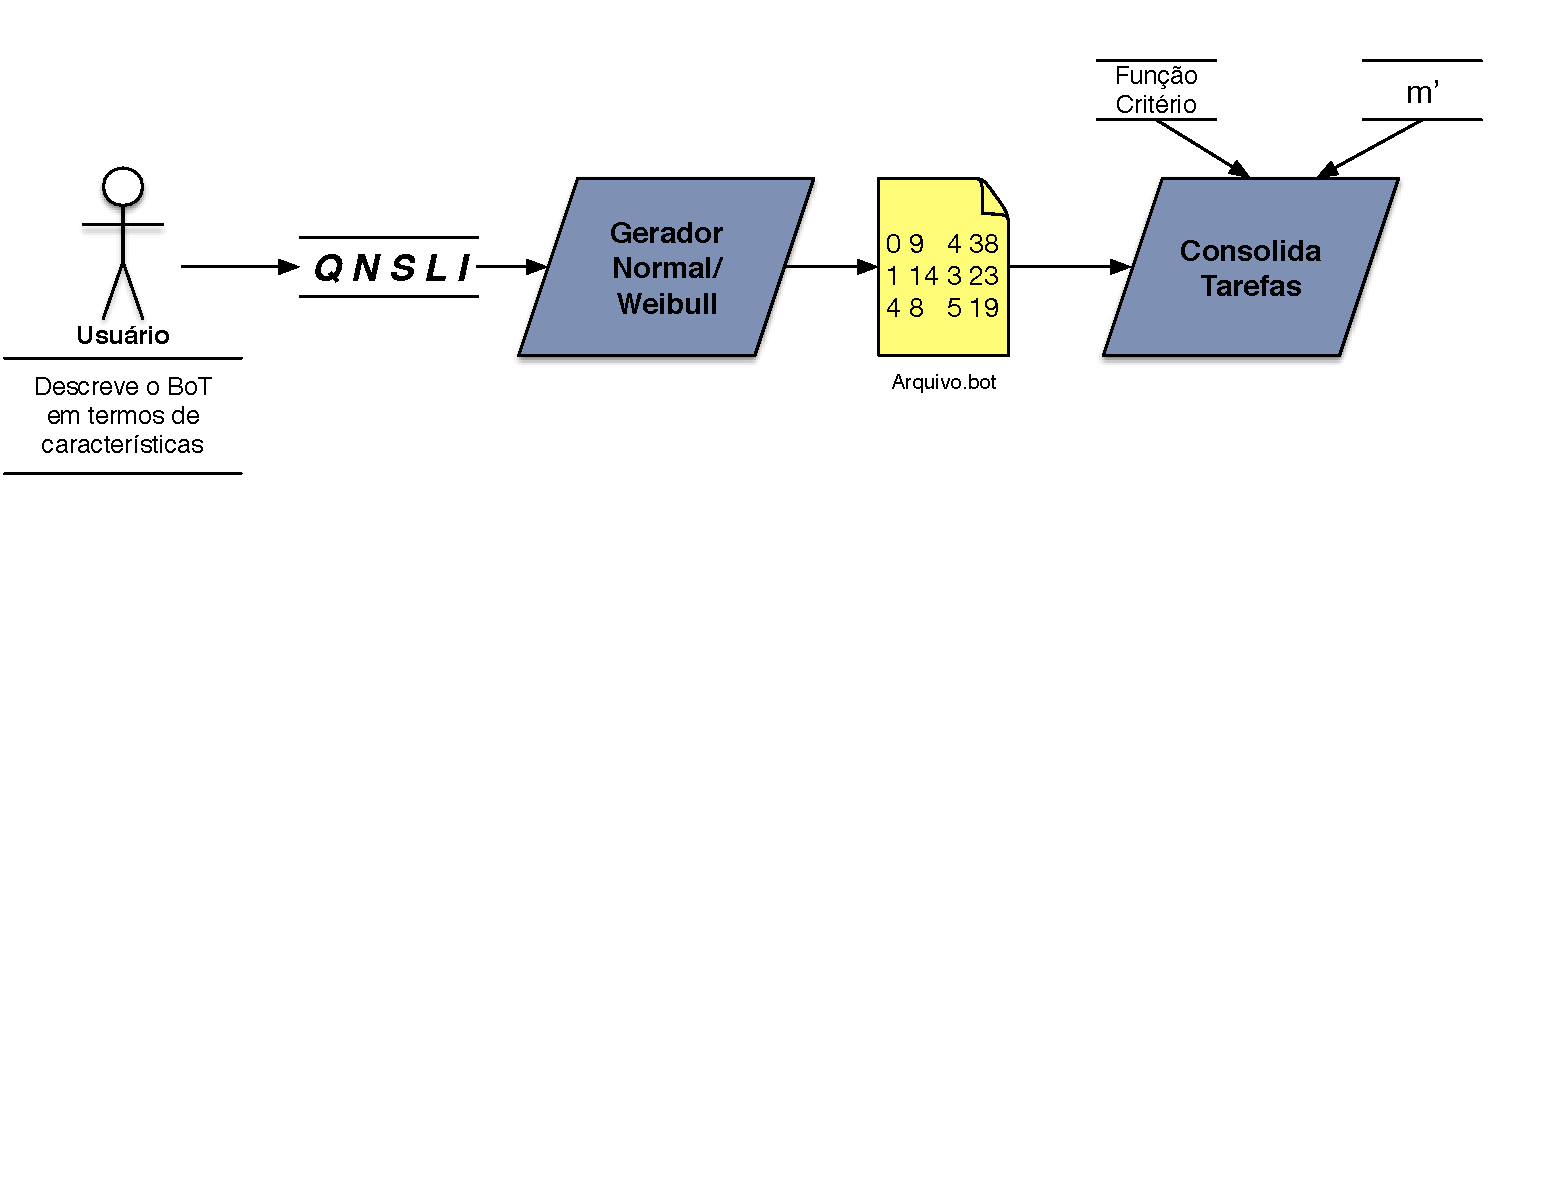
\includegraphics[scale=0.371]{images/ConsolidaTarefas5.pdf}}
%			\caption{Exemplo de descrição de BoT e comsolidação de tarefas.}
%			\label{fig:consolidatarefas5}
%		\end{figure}
%	\end{frame}
%
%	\begin{frame}
%		\begin{figure}[htbp]
%			\centerline{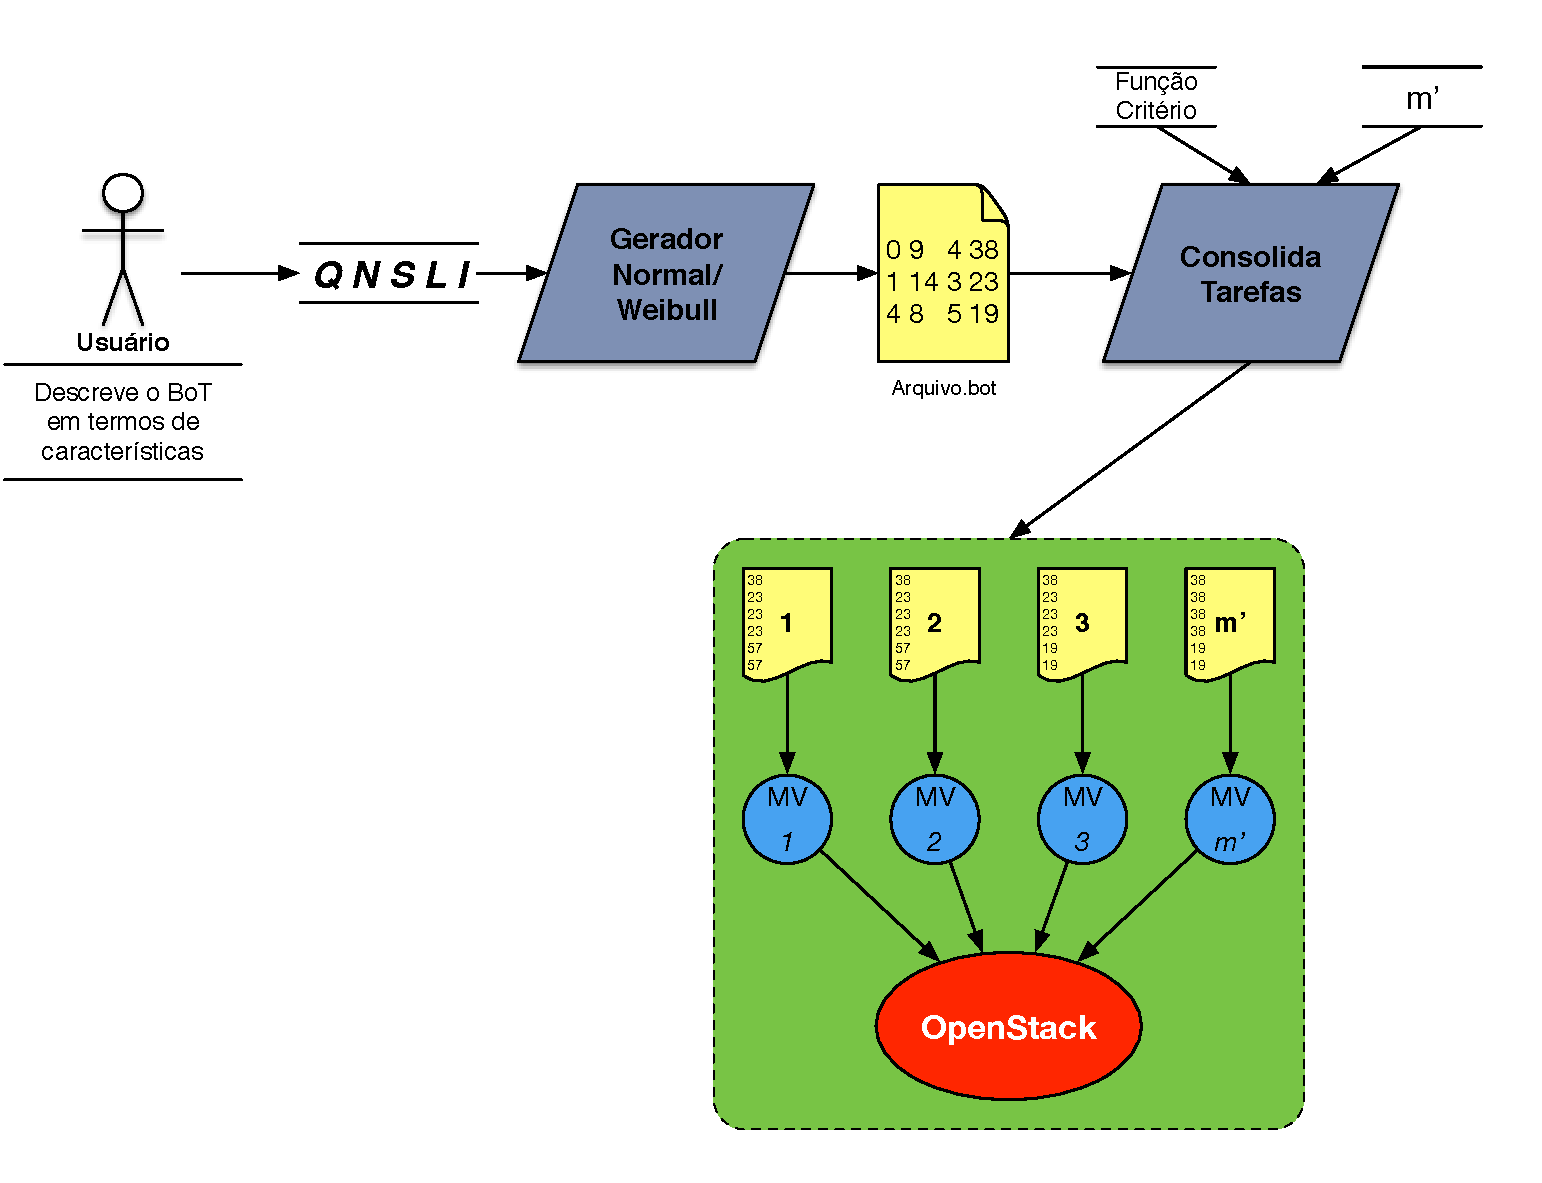
\includegraphics[scale=0.371]{images/ConsolidaTarefas6.pdf}}
%			\caption{Exemplo de descrição de BoT e comsolidação de tarefas.}
%			\label{fig:consolidatarefas6}
%		\end{figure}
%	\end{frame}
%
%	\begin{frame}
%		\begin{figure}[htbp]
%			\centerline{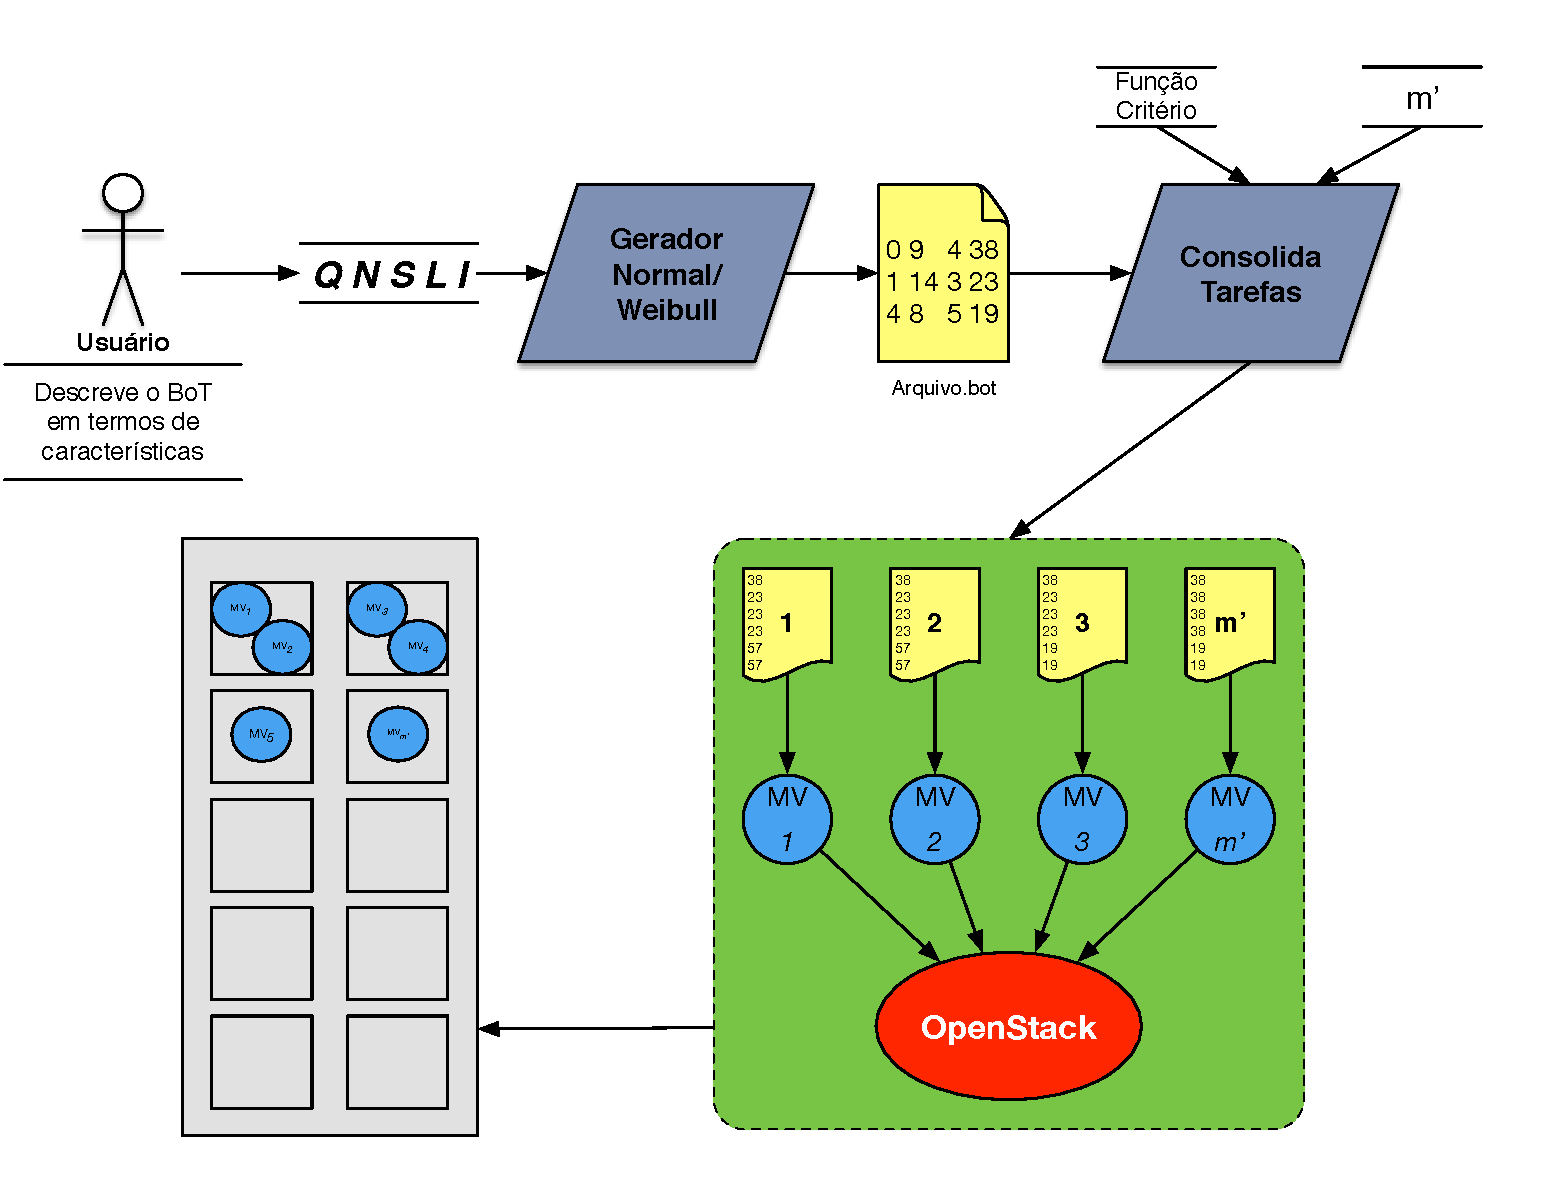
\includegraphics[scale=0.371]{images/ConsolidaTarefas7.pdf}}
%			\caption{Exemplo de descrição de BoT e comsolidação de tarefas.}
%			\label{fig:consolidatarefas7}
%		\end{figure}
%	\end{frame}
%
%\newcommand{\shellcmd}[1]{\\\indent\indent\texttt{\footnotesize\# #1}\\}
%
%	\begin{frame}
%		\begin{block}{Máquinas Virtuais}
%			\begin{itemize}
%				\item[•] Cada máquina virtual foi configurada com 1 (uma) VCPU e 2GB de memória RAM;
%				\item[•] Sistema Operacional Ubuntu 14.04;
%				\item[•] Cada instância virtual executa um script que recupera um arquivo de carga a ser produzida;
%				\item[•] Iterativamente, a carga é realizada com o comando:
%				\item \noindent
%			\shellcmd{stress-ng -c 1 -l \$LOAD --cpu-ops \$BOGO}
%			\end{itemize}
%		\end{block}	
%	\end{frame}
%
%	\subsection*{Casos Triviais}
%	
%	\begin{frame}
%		\begin{center}
%			\begin{huge}
%				\textbf{Casos Triviais}
%			\end{huge}
%		\end{center}
%	\end{frame}
%	
%	\begin{frame}
%		\frametitle{Tarefas leves e muitos recursos de processamento}
%		\begin{center}
%			\begin{block}{Hipótese 1}
%				\textit{Dado um BoT descrito por tarefas com baixo consumo de CPU, havendo uma quantidade suficiente de recursos físicos de processamento, o tempo total de execução real deve ser igual ao tempo de execução em uma arquitetura não contingenciada.}
%			\end{block}
%		\end{center}	
%	\end{frame}
%	
%	\begin{frame}
%		\begin{block}{BoTs gerados para validar Hipótese 1}
%			\begin{center}
%				\begin{tabular}{ll}
%					H1-1 = \( \{ [0, 5, 3, 24], [3, 6, 7, 30] \}\)\\
%					H1-2 = \( \{ [0, 9, 4, 38], [1, 14, 3, 23], [4, 8, 5, 19] \}\)\\
%					H1-3 = \( \{ [0, 11, 5, 18], [2, 4, 8, 15], [5, 6, 4, 29], [6, 4, 2, 25] \}\)\\
%				\end{tabular}
%			\end{center}
%		\end{block}	
%	\end{frame}
%	
%	\begin{frame}
%		\begin{block}{}
%			\begin{table}[htbp]
%				\centering
%				\caption{Tempos de execução, em minutos, para validar Hipótese 1.}
%				\label{tab:casotrivial-1}
%				{\footnotesize
%				\begin{tabular}{cclc}
%					\hline
%					\multicolumn{1}{c|}{\multirow{2}{*}{BoT}} & \multicolumn{2}{c|}{Previsão}       & \multirow{2}{*}{Real} \\ \cline{2-3}
%					\multicolumn{1}{c|}{}                     & Cíclico & \multicolumn{1}{l|}{Lote} &                       \\ \hline
%					H1-1                                      & 45      & 45                        & 45                    \\
%					H1-2                                      & 75      & 75                        & 75                    \\
%					H1-3                                      & 55      & 55                        & 55                    \\ \hline
%				\end{tabular}}
%			\end{table}
%		\end{block}
%	\end{frame}
%	
%	\begin{frame}
%		\frametitle{Tarefas pesadas e poucos recursos de processamento}
%		\begin{center}
%			\begin{block}{Hipótese 2}
%				\textit{Dado um BoT descrito por tarefas com alto consumo de CPU, havendo uma quantidade insuficiente de recursos físicos de processamento, o tempo total de execução real será maior que o tempo de execução em uma arquitetura não contingenciada.}
%			\end{block}
%		\end{center}	
%	\end{frame}
%	
%	\begin{frame}
%		\begin{block}{BoTs gerados para validar Hipótese 2}
%			\begin{center}
%				{\footnotesize
%				\begin{tabular}{ll}
%					H2-1 = \( \{ [0, 5, 3, 84], [3, 6, 7, 90] \}\)\\
%					H2-2 = \( \{ [0, 5, 10, 68], [1, 4, 5, 73], [2, 6, 6, 83], [2, 2, 3, 65], [4, 3, 5, 65] \}\)\\
%					H2-3 = \( \{ [0, 3, 5, 78], [2, 4, 5, 75], [3, 2, 4, 80], [3, 3, 8, 60], [5, 5, 4, 69], [6, 4, 2, 65] \}\)\\
%				\end{tabular}}
%			\end{center}
%		\end{block}
%	\end{frame}
%	
%	\begin{frame}
%		\begin{block}{}
%			\begin{table}[htbp]
%				\centering
%				\caption{Tempos de execução, em minutos, para validar Hipótese 2.}
%				\label{tab:casotrivial-2}
%				{\footnotesize
%				\begin{tabular}{cccccc}
%					\hline
%					\multicolumn{1}{c|}{\multirow{3}{*}{BoT}} & \multicolumn{4}{c|}{Previsão}                                      & \multirow{3}{*}{Real} \\ \cline{2-5}
%					\multicolumn{1}{c|}{}                     & \multicolumn{2}{c|}{Cíclico} & \multicolumn{2}{c|}{Lote}           &                       \\ \cline{2-5}
%					\multicolumn{1}{c|}{}                     & 10 MVs        & 8 MVs        & 10 MVs & \multicolumn{1}{c|}{8 MVs} &                       \\ \hline
%					H2-1                                      & 45            & 55           & 45     & 55                         & 55                    \\
%					H2-2                                      & 140           & 260          & 140    & 260                        & 260                   \\
%					H2-3                                      & 130           & 155          & 130    & 155                        & 155                   \\ \hline
%				\end{tabular}}
%			\end{table}
%		\end{block}
%	\end{frame}
%	
%	\subsection*{Uso em Produção}
%	
%	\begin{frame}
%		\begin{center}
%			\begin{huge}
%				\textbf{Uso em Produção}
%			\end{huge}
%		\end{center}
%	\end{frame}
%	
%	\begin{frame}
%		\begin{block}{}
%			\begin{table}[htbp]
%			\centering
%			\caption{Classes de diferentes BoTs gerados para uso em produção}
%			\label{tab:UP1-10}
%			{\footnotesize
%				\begin{tabular}{lccccc}
%					\hline
%					UP    & \#Quádruplas & \#Tarefas/Quád. & Duração     & Custo         & Intervalo   \\ \hline
%					UP-1  & $Q_5$        & $N^{4}_{2}$     & $S^{3}_{1}$ & $L^{10}_{2}$  & $I^{2}_{1}$ \\
%                    \multicolumn{6}{c}{$\dots$}\\
%					UP-5  & $Q_{10}$     & $N^{4}_{2}$     & $S^{3}_{1}$ & $L^{10}_{2}$  & $I^{2}_{1}$ \\
%                    \multicolumn{6}{c}{$\dots$}\\
%					UP-10 & $Q_{20}$     & $N^{6}_{3}$     & $S^{5}_{1}$ & $L^{50}_{10}$ & $I^{4}_{2}$ \\ \hline
%				\end{tabular}}
%			\end{table}
%		\end{block}
%	\end{frame}
%	
%	\begin{frame}
%		\begin{block}{}
%			\begin{table}[htbp]
%				\centering
%				\caption{Número de tarefas e projeção dos tempos, em minutos, de execução de BoTs em produção considerando diferentes números de MVs.}
%				\label{tab:UPsConsolidados}
%				\resizebox{\textwidth}{!}{%
%				\begin{tabular}{ccccccccc}
%					\hline
%					\multirow{2}{*}{BoT} & \multirow{2}{*}{\#Tarefas} & \multicolumn{1}{c|}{\multirow{2}{*}{Arrival Time}} & \multicolumn{2}{c|}{Previsão 16 MVs} & \multicolumn{2}{c|}{Previsão 20 MVs} & \multicolumn{2}{c}{Previsão 36 MVs} \\ \cline{4-9} 
%				 &  & \multicolumn{1}{c|}{} & \multicolumn{1}{c|}{Cíclico} & \multicolumn{1}{c|}{Lote} & \multicolumn{1}{c|}{Cíclico} & \multicolumn{1}{c|}{Lote} & \multicolumn{1}{c|}{Cíclico} & Lote \\ \hline
%					UP-10 & 89 & 0 & 275 & 275 & 275 & 275 & 275 & 275 \\
%					UP-5 & 23 & 33 & 60 & 60 & 60 & 60 & 60 & 60 \\
%					UP-1 & 8 & 54 & 25 & 25 & 25 & 25 & 25 & 25 \\\hline
%					UP-1 a UP-10 & 318 & 0 & 770 & 640 & 640 & 490 & 490 & 490 \\ \hline
%				\end{tabular}%
%				}
%			\end{table}
%		\end{block}
%	\end{frame}
%	
%	\begin{frame}
%		\begin{block}{}
%			\begin{table}[htbp]
%				\centering
%				\caption{Tempo real, em minutos, de execução de BoTs em produção considerando diferente número de MVs em uma infraestrutura dedicada.}
%				\label{my-label}
%				{\footnotesize
%				\begin{tabular}{lccc}
%					\cline{2-4}
%					 & 16 MVs & 20 MVs & 36 MVs \\ \hline
%					Infraestrutura ociosa & 883 & 733 & 553 \\
%					Infraestrutura 50\% & 819 & 684 & 527 \\
%					Infraestrutura 75\% & 825 & 691 & 540 \\ \hline
%				\end{tabular}}
%			\end{table}
%		\end{block}
%	\end{frame}
%	
%	\subsection*{Impacto em Perfis de Usuários}
%	
%	\begin{frame}
%		\begin{center}
%			\begin{huge}
%				\textbf{Impacto em Perfis de Usuários}
%			\end{huge}
%		\end{center}
%	\end{frame}
%	
%	\begin{frame}
%		\begin{block}{}
%			\begin{table}[htbp]
%				\centering
%				\caption{Configuração de BoTs com diferentes perfis de carga de processamento: Leve, Mediano e Pesado.}
%				\label{tab:ConfiguracaoPerfis}
%				{\footnotesize
%				\begin{tabular}{lccccccc}
%					\hline
%					\multicolumn{1}{c|}{\multirow{2}{*}{BoT}} & \multicolumn{5}{c|}{Classe} & \multirow{2}{*}{\#Tarefas} & \multirow{2}{*}{MVs} \\ \cline{2-6}
%					\multicolumn{1}{c|}{} & \multicolumn{1}{c|}{$Q$} & \multicolumn{1}{c|}{$N$} & \multicolumn{1}{c|}{$S$} & \multicolumn{1}{c|}{$L$} & \multicolumn{1}{c|}{$I$} &  &  \\ \hline
%					Leve & $Q_{10}$ & $N^{10}_{4}$ & $S^{3}_{1}$ & $L^{10}_{2}$ & $I^{2}_{1}$ & 74 & 3 \\
%					Mediano & $Q_{10}$ & $N^{10}_{4}$ & $S^{3}_{1}$ & $L^{50}_{10}$ & $I^{2}_{1}$ & 74 & 24 \\
%					Pesado & $Q_{10}$ & $N^{10}_{4}$ & $S^{3}_{1}$ & $L^{75}_{20}$ & $I^{2}_{1}$ & 74 & 24 \\ \hline
%				\end{tabular}}
%			\end{table}
%		\end{block}
%	\end{frame}
%
%	\begin{frame}
%		\begin{block}{}
%			\begin{table}[htbp]
%				\centering
%				\caption{Tempo real de execução, com diferentes taxas de sobrecarga da infraestrutura.}
%				\label{my-label}
%				\resizebox{\textwidth}{!}{%
%				{\tiny
%				\begin{tabular}{lccccccc}
%					\hline
%					\multicolumn{1}{c}{\multirow{2}{*}{Perfil}} & \multicolumn{1}{c|}{\multirow{2}{*}{Cíclico}} & \multicolumn{3}{c|}{Ocupação da Infraestrutura} & \multicolumn{3}{c}{Diferença} \\ \cline{3-8} 
%					\multicolumn{1}{c}{} & \multicolumn{1}{c|}{} & \multicolumn{1}{c|}{Ocioso} & \multicolumn{1}{c|}{50\%} & \multicolumn{1}{c|}{75\%} & \multicolumn{1}{c|}{Ocioso} & \multicolumn{1}{c|}{50\%} & 75\% \\ \hline
%					Leve & 80 & 93 & 86 & 86 & 16,25\% & 7,5\% & 7,5\% \\
%					Mediano & 65 & 75 & 74 & 78 & 15,4\% & 13,8\% & 20\% \\
%					Pesado & 75 & 83 & 89 & 96 & 10,7\% & 18,7\% & 28\% \\ \hline
%				\end{tabular}}%
%				}
%			\end{table}
%			
%			\begin{table}[htbp]
%				\centering
%				\caption{Tempo real de execução, com escalonamento sistema.}
%				\label{my-label}
%				\resizebox{\textwidth}{!}{%
%				{\tiny
%				\begin{tabular}{lccccccc}
%					\hline
%					\multicolumn{1}{c}{\multirow{2}{*}{Perfil}} & \multicolumn{1}{c|}{\multirow{2}{*}{Cíclico}} & \multicolumn{3}{c|}{Ocupação da Infraestrutura} & \multicolumn{3}{c}{Diferença} \\ \cline{3-8} 
%					\multicolumn{1}{c}{} & \multicolumn{1}{c|}{} & \multicolumn{1}{c|}{Ocioso} & \multicolumn{1}{c|}{50\%} & \multicolumn{1}{c|}{75\%} & \multicolumn{1}{c|}{Ocioso} & \multicolumn{1}{c|}{50\%} & 75\% \\ \hline
%					Leve & 80 & 92 & 86 & 86 & 15\% & 7,5\% & 7,5\% \\
%					Mediano & 65 & 74 & 77 & 86 & 13,8\% & 18,5\% & 32,3\% \\
%					Pesado & 75 & 84 & 94 & 90 & 12\% & 25,3\% & 20\% \\ \hline
%				\end{tabular}}%
%				}
%			\end{table}			
%		\end{block}
%	\end{frame}

\section[Conclusão]{Conclusão}

\begin{frame}
	\tableofcontents[currentsection]
\end{frame}

\begin{frame}
	\frametitle{Conclusão}
	\begin{block}{}
		\begin{itemize}
			\item[•] Revisão das questões de seleção de serviços em nuvam, considerando diferentes abordagens CSB;
			\newline
			\item[•] Nenhuma abordagem investigada suporta todos os atributos propostos para um CSB efetivo; 
		\end{itemize}
	\end{block}
\end{frame}

\begin{frame}
	\frametitle{Conclusão}
	\begin{block}{}
		\begin{itemize}
			\item[•] Na teoria é possível, porém, torna-se impraticável um CSB que suporte todos os atributos;
			\newline
			\item[•] É necessário priorizar os atributos a fim de encontar um equilíbrio e selecionar os que melhor se conformam ao objetivo do CSB.
		\end{itemize}
	\end{block}
\end{frame}

%\begin{frame}
%	\frametitle{}
%	\begin{block}{Dados sobre o artigo}
%		\begin{itemize}
%			\item[•] 
%			\item[•] 
%			\item[•] Fator de Impacto 2017: 1.105
%		\end{itemize}
%	\end{block}
%	\begin{varblock}[4cm]{New block}
%  Variable width, here 4cm
%\end{varblock}
%\end{frame}

\begin{frame}{Dados do Artigo}
\begin{minipage}{0.47\textwidth}
		\begin{itemize}
			\item[•] Accepted Date: 10/05/2017
			\item[•] Online Date: 13/06/2018
			\item[•] FI 2017: 1.105 (\textit{journal})
		\end{itemize}
\end{minipage}
\begin{minipage}{0.5\textwidth}
    \begin{figure}[htbp]
		\centerline{
\includegraphics[scale=0.15]{images/fcs.jpg}}
			\label{fig:consolidatarefas6}
		\end{figure}
\end{minipage}
Acesso: \url{http://journal.hep.com.cn/fcs/EN/10.1007/s11704-017-6124-7}
\end{frame}

%\section{Referências}
%
%\begin{frame}
%	\tableofcontents[currentsection]
%\end{frame}
%
%\begin{frame}[allowframebreaks]
%	\frametitle{Referências}
%	\def\newblock{}
%	\bibliographystyle{plain}
%	\tiny \bibliography{bibliografia}
%\end{frame}

%\section*{Agradecimentos}
%	
%\begin{frame}
%	\begin{center}
%		\textbf{Obrigado!}
%	\end{center}
%	\begin{figure}[htbp]
%		\begin{center}
%			
\includegraphics[scale=.09]{images/Question-Mark.jpg}
%		\end{center}
%	\end{figure}
%	\begin{center}
%		\url{madsantos@inf.ufpel.edu.br}
%	\end{center}
%\end{frame}

%%%%%%%%%%%%%%%%%%%%%%%%%%%%%%%%%%%%%%%%%%%%
% Último Slide
%%%%%%%%%%%%%%%%%%%%%%%%%%%%%%%%%%%%%%%%%%%%
\frame
{
	\pgfdeclareimage[height=1.5cm]{logo}{images/lups_oficial.png}
	\logo{\pgfuseimage{logo}
}	
	\logo{\vspace{3mm} 
	\begin{large}
		\textbf{Obrigado!} 
	\end{large}}
	\titlepage
}

\end{document}